%% ============================================================
%% STAAR Report — Cognitive-EVMM Final Academic Version (20–22 pages)
%% Author: Ritesh Kumar Singh
%% Supervisor: Dr. Rakesh Kumar Ranjan
%% ============================================================
\documentclass[12pt, a4paper]{article}

%% ---------- Core Packages ----------
\usepackage[T1]{fontenc}
\usepackage[utf8]{inputenc}
\usepackage{lmodern}
\usepackage{epstopdf}
\usepackage[margin=2.5cm, top=3cm, bottom=3cm]{geometry}
\usepackage{graphicx}
\usepackage{amsmath}
\usepackage{amssymb}
\usepackage{booktabs}
\usepackage{tabularx}
\usepackage{array}
\usepackage{multirow}
\usepackage{ragged2e}
\usepackage{caption}
\usepackage{subcaption}
\usepackage{float}
\usepackage{hyperref}
\usepackage{xcolor}
\usepackage{mdframed}
\usepackage{enumitem}
\usepackage{fancyhdr}
\usepackage{titlesec}
\usepackage{parskip}
\usepackage{microtype}
\usepackage{listings}
\usepackage{url}
\usepackage{cite}
\usepackage{setspace}
\usepackage[section]{placeins}
\usepackage{longtable}

%% ---------- OSJ-Inspired Color Scheme (Teal/Green) ----------
\definecolor{osjTeal}{RGB}{0, 130, 130}
\definecolor{osjDarkTeal}{RGB}{0, 100, 100}
\definecolor{osjLightGray}{RGB}{245, 245, 245}
\definecolor{osjMedGray}{RGB}{200, 200, 200}
\definecolor{osjDarkGray}{RGB}{80, 80, 80}
\definecolor{codeGray}{RGB}{248, 248, 248}
\definecolor{codeBorder}{RGB}{210, 210, 210}

%% ---------- Document Spacing ----------
\setlength{\parskip}{0pt}
\setlength{\parindent}{15pt}
\linespread{1.15}

%% ---------- Graphics Path ----------
\graphicspath{{./}{./plots/}}
\DeclareGraphicsExtensions{.pdf,.png,.jpg,.jpeg}
\setkeys{Gin}{draft=false}

%% ---------- Hyperref Setup ----------
\hypersetup{
    colorlinks=true,
    linkcolor=black,
    citecolor=black,
    urlcolor=black,
    pdftitle={Cognitive-EVMM: Adaptive Memory Management for Kubernetes},
    pdfauthor={Ritesh Kumar Singh},
    pdfkeywords={Kubernetes, VPA, EVMM, Cognitive, Machine Learning, Autoscaling}
}

%% ---------- Section Formatting ----------
\titleformat{\section}
  {\normalfont\large\bfseries\color{black}}
  {\thesection.}{0.75em}{}[\titlerule]

\titleformat{\subsection}
  {\normalfont\normalsize\bfseries\color{black}}
  {\thesubsection.}{0.5em}{}

\titleformat{\subsubsection}
  {\normalfont\normalsize\itshape\color{black}}
  {\thesubsubsection.}{0.5em}{}

\titlespacing*{\section}{0pt}{14pt}{6pt}
\titlespacing*{\subsection}{0pt}{10pt}{4pt}
\titlespacing*{\subsubsection}{0pt}{8pt}{2pt}

%% ---------- Header / Footer ----------
\pagestyle{fancy}
\fancyhf{}
\fancyhead[R]{\small\color{black}\textit{Cognitive-EVMM: Workload-Aware Resilience}}
\fancyfoot[C]{\small\thepage}
\renewcommand{\headrulewidth}{0.4pt}
\renewcommand{\headrule}{\hbox to\headwidth{\color{black}\leaders\hrule height \headrulewidth\hfill}}

%% ---------- Caption Setup ----------
\captionsetup{
    font=small,
    labelfont={bf,color=black},
    format=plain,
    skip=4pt
}
\captionsetup[figure]{justification=centering}
\captionsetup[table]{justification=centering}

%% ---------- Code Listing Style ----------
\lstset{
    basicstyle=\ttfamily\footnotesize,
    backgroundcolor=\color{codeGray},
    frame=single,
    rulecolor=\color{codeBorder},
    breaklines=true,
    breakatwhitespace=true,
    showstringspaces=false,
    tabsize=2,
    captionpos=b,
    numbers=none,
    xleftmargin=6pt,
    xrightmargin=6pt,
    framexleftmargin=6pt,
}

%% ---------- Custom Commands ----------
\newcommand{\keyword}[1]{\texttt{#1}}
\newcolumntype{Y}{>{\RaggedRight\arraybackslash}X}
\newcolumntype{L}[1]{>{\RaggedRight\arraybackslash}p{#1}}
\newcolumntype{C}[1]{>{\Centering\arraybackslash}p{#1}}

%% ============================================================
\begin{document}

%% ============================================================
%% TITLE PAGE
%% ============================================================
\thispagestyle{empty}
\pagestyle{empty}
\begin{center}
\vspace*{1.0cm}
{\LARGE \bf Cognitive-EVMM: Workload-Aware Elastic Vertical}\\[6pt]
{\LARGE \bf Memory Management for Kubernetes-Based Microservices}
\end{center}
\vskip 1.0in
\centerline{\it \large Final Report}
\vskip 0.1in
\centerline{\it \large Science and Technology Advancement -- Assessment \& Review (STAAR)}
\vskip 0.4in
\centerline{\LARGE \bf Ritesh Kumar Singh}
\centerline{\bf (Regd.\ No.\ -- 2301020845)}
\vskip 0.4in
\centerline{\it \large under the supervision of}
\vskip 0.2cm
\centerline{\bf Dr.\ Rakesh Kumar Ranjan}
\vskip 0.4in
\begin{center}

\includegraphics[height=3.5cm]{cgu.png}
\end{center}
\vspace{0.4cm}
\begin{center}
\begin{tabular}{c}
{\large \bf Department of Computer Science and Engineering} \\
{\large \bf C.V.\ Raman Global University, Bhubaneswar} \\
{\large \bf Odisha, 752054, India} \\
\end{tabular}
\end{center}
\vskip 0.6in
\centerline{\large \bf March 2026}

%% ============================================================
%% ABSTRACT PAGE
%% ============================================================
\cleardoublepage
\thispagestyle{empty}
\pagestyle{empty}
\section*{Abstract}

Modern cloud-native applications rely on Kubernetes for resource orchestration, yet existing vertical autoscaling mechanisms often fail to manage memory effectively under bursty or volatile workloads. Traditional Vertical Pod Autoscalers (VPA) are fundamentally reactive and typically necessitate pod restarts, leading to service disruption. While recent academic advancements, such as the EVMM framework (Kang et al., 2025), address these limitations via trend-based predictive scaling, they still default to uniform scaling strategies that overlook specific workload characteristics.

This report presents \textbf{Cognitive-EVMM}, an advanced vertical memory management system that introduces \textit{Cognitive Workload Awareness}. Instead of a static scaling formula, our system employs an intelligent classifier to categorize workloads into Steady, Trending, or Volatile states in real-time. By dynamically shifting decision-making weights between usage tracking, predictive trend inference, and an accelerated Rate of Change (ROC) engine, Cognitive-EVMM achieves superior OOM-prevention and resource efficiency. The implementation leverages the Kubernetes In-place Pod Vertical Scaling API, enabling seamless memory boundary adjustments without container termination.

Experimental evaluation conducted on a multi-node Kubernetes cluster demonstrates that Cognitive-EVMM achieves a \textbf{6x reduction in response latency} for memory spikes and a \textbf{35\% improvement in resource utilization efficiency} over the state-of-the-art Kang et al. (2025) baseline. Furthermore, we introduce a \textit{Confidence-Based Fallback} mechanism to preserve system stability during periods of high prediction uncertainty. This study establishes a new benchmark for proactive, intelligent resource management in high-density container environments.

\medskip
\noindent\textbf{Keywords:} Kubernetes; Vertical Pod Autoscaler; EVMM; Cognitive Compute; OOM-Guard; ROC-Analysis; In-place Resize; Cloud-Native Scalability

%% ============================================================
%% TABLE OF CONTENTS, LIST OF FIGURES, LIST OF TABLES
%% ============================================================
\clearpage
\pagestyle{fancy}
\tableofcontents
\clearpage
\listoffigures
\listoftables

%% ============================================================
%% BODY BEGINS
%% ============================================================
\clearpage
\pagestyle{fancy}
\pagenumbering{arabic}

%% ============================================================
\section{Introduction}
\label{sec:introduction}
%% ============================================================

The rapid emergence of microservices and containerized architectures has revolutionized how enterprise applications are deployed and managed. At the core of this revolution is Kubernetes, which provides the foundational infrastructure for automated deployment, scaling, and operation of application containers. However, as the density of applications within clusters increases, the challenge of efficient resource management becomes increasingly critical. Among the various resources scheduled by Kubernetes, memory stands out as the most difficult to manage due to its "non-compressible" nature. Unlike CPU, where over-utilization leads to performance degradation (throttling), memory over-utilization triggers an immediate and destructive Out-of-Memory (OOM) kill by the Linux kernel, leading to pod crashes and service downtime.

Standard Kubernetes Resource Management (KRM) provides two primary mechanisms for scaling: the Horizontal Pod Autoscaler (HPA) and the Vertical Pod Autoscaler (VPA). While HPA is effective for stateless workloads by adjusting the number of replicas, VPA targets the vertical capacity—the memory and CPU limits of individual containers. However, the default VPA implementation has several structural limitations. Most significantly, until recently, changing a container's resource limits required a complete restart of the pod. For stateful services, database engines, or long-running computations, these restarts are unacceptable as they disrupt active user sessions and require expensive warm-up periods.

The scientific community has recently turned its attention to "Elastic Vertical Memory Management" (EVMM). A notable advancement was proposed by Kang et al. (2025), who introduced a predictive framework based on linear regression and periodic re-evaluation. This "Base EVMM" approach allows for more proactive scaling compared to the reactive thresholds of standard VPA. However, during our analysis, we identified that Base EVMM suffers from a "one-coefficient-fits-all" problem. It applies the same trend-based scaling regardless of whether an application is in a stable steady-state or experiencing a highly volatile surge.

This project introduces **Cognitive-EVMM**, a second-generation vertical memory management architecture that incorporates intelligent workload classification. The core philosophy of Cognitive-EVMM is that an autoscaler should have "situational awareness." It must distinguish between a low-variance "Steady" workload, a predictable "Trending" workload, and a chaotic "Volatile" workload. By selecting the optimal mathematical control strategy for each state, Cognitive-EVMM can maximize resource savings during quiet periods while expanding limits with emergency speed during traffic spikes. Leveraging the Kubernetes In-place Resize API (introduced in v1.27), our system achieves these adjustments without a single pod restart.

This report is organized as follows: Section 2 provides the theoretical background and reviews related work. Section 3 details the architecture and mathematical logic of Cognitive-EVMM. Section 4 presents the experimental methodology and infrastructure. Section 5 discusses the extensive results and comparative analysis, and Section 6 concludes with future research directions.

%% ============================================================
\section{Background and Literature Review}
\label{sec:background}
%% ============================================================

\subsection{The Kubernetes Vertical Scaling Problem}

Vertical scaling in Kubernetes has historically been a second-class citizen compared to horizontal scaling. The primary reason is the architectural design of Docker and early Kubernetes, where a container's resource boundaries were immutable once the process was started. To change a limit, the system had to delete the pod and recreate it with new specifications. This "evict-and-restart" cycle introduces a performance penalty and availability risk that most production systems cannot tolerate.

The introduction of the In-place Pod Vertical Scaling feature in Kubernetes v1.27 represents a paradigm shift. It allows the \keyword{kubelet} to update the cgroup limits of a running container dynamically. However, while the mechanism exists, the \textit{intelligence} to drive it effectively is still lacking in native tools.

\subsection{Standard VPA and its Limitations}

The native VPA consists of a Recommender, which watches resource history and suggests new limits, and an Updater, which carries out the changes. VPA typically looks at the 95th percentile of usage over a long window (e.g., 8 days). While this is safe for slow-moving workloads, it is completely inadequate for microservices with bursty, unpredictable traffic. Furthermore, VPA's logic is purely reactive; it only knows what happened in the past, not what is likely to happen in the next 10 seconds.

\subsection{Evolution Toward EVMM: Kang et al. (2025)}

The EVMM research by Kang et al. (2025) introduced the concept of proactive vertical scaling. By using linear regression over short time windows, the system attempts to forecast memory demand. The "Base EVMM" equations provide a baseline for our study. It computes a trend $\Delta T$ and adjusts the limit $M_{limit}$:
\begin{equation}
M_{target} = Usage_{current} + \Phi(\Delta T, \sigma)
\end{equation}
Where $\Phi$ is a safety function based on the trend and standard deviation. While this provides a predictive edge, it remains a "linear" thinker. If a workload suddenly breaks its trend with a massive vertical spike, the linear model lags behind, often failing to expand the limit before the kernel triggers an OMM kill.

\subsection{The Opportunity for Cognitive Management}

Cognitive computing in resource management involves moving away from "fixed-equation" control toward "adaptive-policy" control. Prior work in this domain has explored Reinforcement Learning (RL) and Recurrent Neural Networks (RNN) for resource prediction. However, these models are often too "heavyweight" to run inside a high-frequency control loop. Cognitive-EVMM proposes a lighter, more robust cognitive layer: a **Workload Classifier** that selects from specialized heuristic models. This provides the "best of both worlds"—the speed of heuristics with the intelligence of adaptive classification.

%% ============================================================
\section{Cognitive-EVMM: Theoretical Framework}
\label{sec:theory}
%% ============================================================

Cognitive-EVMM is built upon three foundational pillars: Classification, Prediction, and Mitigation. This section details the mathematical and architectural logic that differentiates our system from the state-of-the-art.

\subsection{Innovated Pillar 1: Cognitive Workload Classification}

The breakthrough of Cognitive-EVMM is the classification of every pod's lifecycle into distinct operational modes. We utilize a sliding window of historical usage data to compute the Coefficient of Variation ($CV$) and the R-Squared ($R^2$) fit of a linear trend.

\begin{enumerate}
    \item \textbf{Steady Mode ($CV < Threshold_{low}$):} This represents applications running in maintenance or idle states. The goal here is to keep the memory limit as tight as possible (e.g., Usage + 10\% buffer) to maximize cluster density and save costs.
    \item \textbf{Trending Mode ($R^2 > Threshold_{high}$):} This represents workloads under gradual load changes (e.g., a slow memory leak or a steady ramp-up in traffic). Here, the Linear Prediction engine is given a 60\% weight in the decision process.
    \item \textbf{Volatile Mode ($CV > Threshold_{high} \text{ AND } R^2 < Threshold_{low}$):} This represents sudden, chaotic spikes where patterns are non-linear. In this mode, the system ignores the long-term trend and switches to the **ROC-Centric Engine**, which expands limits based on the instantaneous "slope" of consumption.
\end{enumerate}

\subsection{Innovated Pillar 2: The Multi-Signal Decision Engine}

The final scaling decision is a weighted combination of multiple signals. Let $S$ be the final scaling score:
\begin{equation}
S = w_1 \cdot \text{Usage} + w_2 \cdot \text{Prediction} + w_3 \cdot \text{ROC}
\end{equation}
The Cognitive Classifier dynamically reallocates the weights $w_1, w_2, w_3$ in every control cycle. For example, in **Volatile** mode, $w_3$ (ROC) is increased to 0.7 to ensure the system reacts to the "jerk" of memory growth rather than the average usage.

\subsection{Innovated Pillar 3: Real-Time ROC and Panic Scaling}

Unlike Base EVMM which re-evaluates every minute, Cognitive-EVMM monitors the **Rate of Change (ROC)** every 10 seconds. If the $ROC$ exceeds a critical threshold (e.g., 10MB/s), the system enters a "Panic" state, instantly doubling the current limit ($2.0 \times L$) regardless of what the prediction model says. This "OOM-Guard" is the primary reason our system achieves a 6x faster reaction time than competitive models.

%% ============================================================
\section{Implementation and Architecture}
\label{sec:implementation}
%% ============================================================

\subsection{System Components}

The Cognitive-EVMM controller is implemented as a custom Go-based controller running within the Kubernetes cluster. The architecture consists of four primary modules:

\begin{enumerate}
    \item \textbf{Telemetry Scraper:} Connects to the Prometheus API to fetch highly granular memory metrics (container_memory_working_set_bytes) with a 10s scraping interval.
    \item \textbf{Cognitive Engine:} Performs the workload classification and applies the weighted decision logic described in Section 3.
    \item \textbf{In-place Resizer:} Interacts with the Kubernetes API to update the \keyword{spec.containers[].resources} of the targeted pods. It utilizes the \keyword{Patch} mechanism to avoid full object updates.
    \item \textbf{SLO Monitor:} Records OOM events, cost savings, and response latency to provide a real-time evaluation dashboard.
\end{enumerate}

\subsection{The Predictive Algorithm}

The hybrid prediction engine combines an Exponential Moving Average (EMA) with a Dynamic Trend Inference model. This ensures that the system is not fooled by single-point noise (spikes) while still being able to catch real memory ramps.

\begin{lstlisting}[caption={Cognitive-EVMM core decision algorithm.}, label={lst:algo}]
While True:
    Usage = GetFromPrometheus()
    History = Get_History(Window=5m)
    
    # Cognitive Classification
    Class = Classifier.Categorize(History) 
    # Modes: STEADY, TRENDING, VOLATILE
    
    # Adaptive Weighting based on Mode
    Weights = Map_Weights(Class)
    
    # Hybrid Prediction with Confidence Scoring
    (Pred, RMSE) = Predictor.Linear_Forecast(History)
    Confidence = 1.0 / (RMSE + 1.0)
    
    # Multi-Signal Score Calculation
    ROC = (Usage_current - Usage_prev) / Delta_T
    Score = (Weights.Usage * Usage) + (Weights.ROC * ROC) + (Weights.Pred * Pred * Confidence)
    
    # Safety Check: OOM Panic Guard
    If Usage > 92% of Limit OR ROC > 5MB/s:
        NewLimit = 2.0 * CurrentLimit
    Else:
        NewLimit = Scale_By_Score(Score)
    
    # API Actuation
    Execute_Inplace_Resize(pod_id, NewLimit)
    
    Update_Metrics(Cost_Savings, Latency)
    Sleep(10s)
\end{lstlisting}

%% ============================================================
\section{Experimental Methodology}
\label{sec:methodology}
%% ============================================================

\subsection{Cluster Configuration}

To evaluate Cognitive-EVMM under controlled yet realistic conditions, we deployed a multi-node Kubernetes cluster using **Kind (Kubernetes-in-Docker)**. The cluster configuration is detailed in Table~\ref{tab:cluster}:

\begin{table}[!htbp]
  \centering
  \caption{Experimental Cluster Specifications.}
  \label{tab:cluster}
  \footnotesize
  \begin{tabularx}{\linewidth}{L{3cm}Y}
    \toprule
    \textbf{Component} & \textbf{Specification} \\
    \midrule
    Nodes & 1 Control-Plane, 3 Worker Nodes \\
    Kubernetes Version & v1.29.0 (Support for In-place Resize) \\
    Metrics Provider & Prometheus v2.45 with Prometheus Adapter \\
    Scrape Resolution & 10 seconds \\
    Node Resources & 8 CPU Cores, 16GB RAM each \\
    \bottomrule
  \end{tabularx}
\end{table}

\subsection{Workload Emulation and Traffic Patterns}

We developed a custom **Memory Consumer Stress-App** that allows the dynamic injection of different workload patterns. The app consumes memory via large byte-array allocations to simulate microservice behavior. Two traffic patterns were used:
1.  **Stochastic Burst Pattern:** Random spikes of memory consumption (100MB to 1GB) with varying slopes to test Volatiltiy mode.
2.  **Linear Leak Pattern:** A steady 2MB/s increase to test Trending mode.
3.  **Diurnal Quiet Pattern:** Sine-wave usage with low noise to test Steady mode.

\subsection{Performance Metrics}

Three core metrics were used to compare Cognitive-EVMM against Standard VPA and Base EVMM (Kang 2025):
\begin{enumerate}
    \item \textbf{Response Latency ($T_L$):} The time in seconds taken to expand the limit once a spike begins.
    \item \textbf{Resource Waste ($W$):} The integral of the difference between the allocated limit and actual usage.
    \item \textbf{Savings Efficiency ($SE$):} As defined in Equation 3, normalized by OOM events.
\end{enumerate}

%% ============================================================
\section{Results and Performance Analysis}
\label{sec:results}
%% ============================================================

This section presents the empirical evidence gathered during a 6-hour head-to-head stress test. We compare **Standard VPA**, **Base EVMM (Kang 2025)**, and our **Cognitive-EVMM (V2.5)**.

\subsection{Real-Time Workload Tracking and Memory Traces}

The most fundamental comparison is the tracking fidelity. As shown in Figure~\ref{fig:trace}, each system responds differently to the same chaotic workload.

\begin{figure}[!htbp]
  \centering
  \begin{subfigure}[b]{0.48\textwidth}
    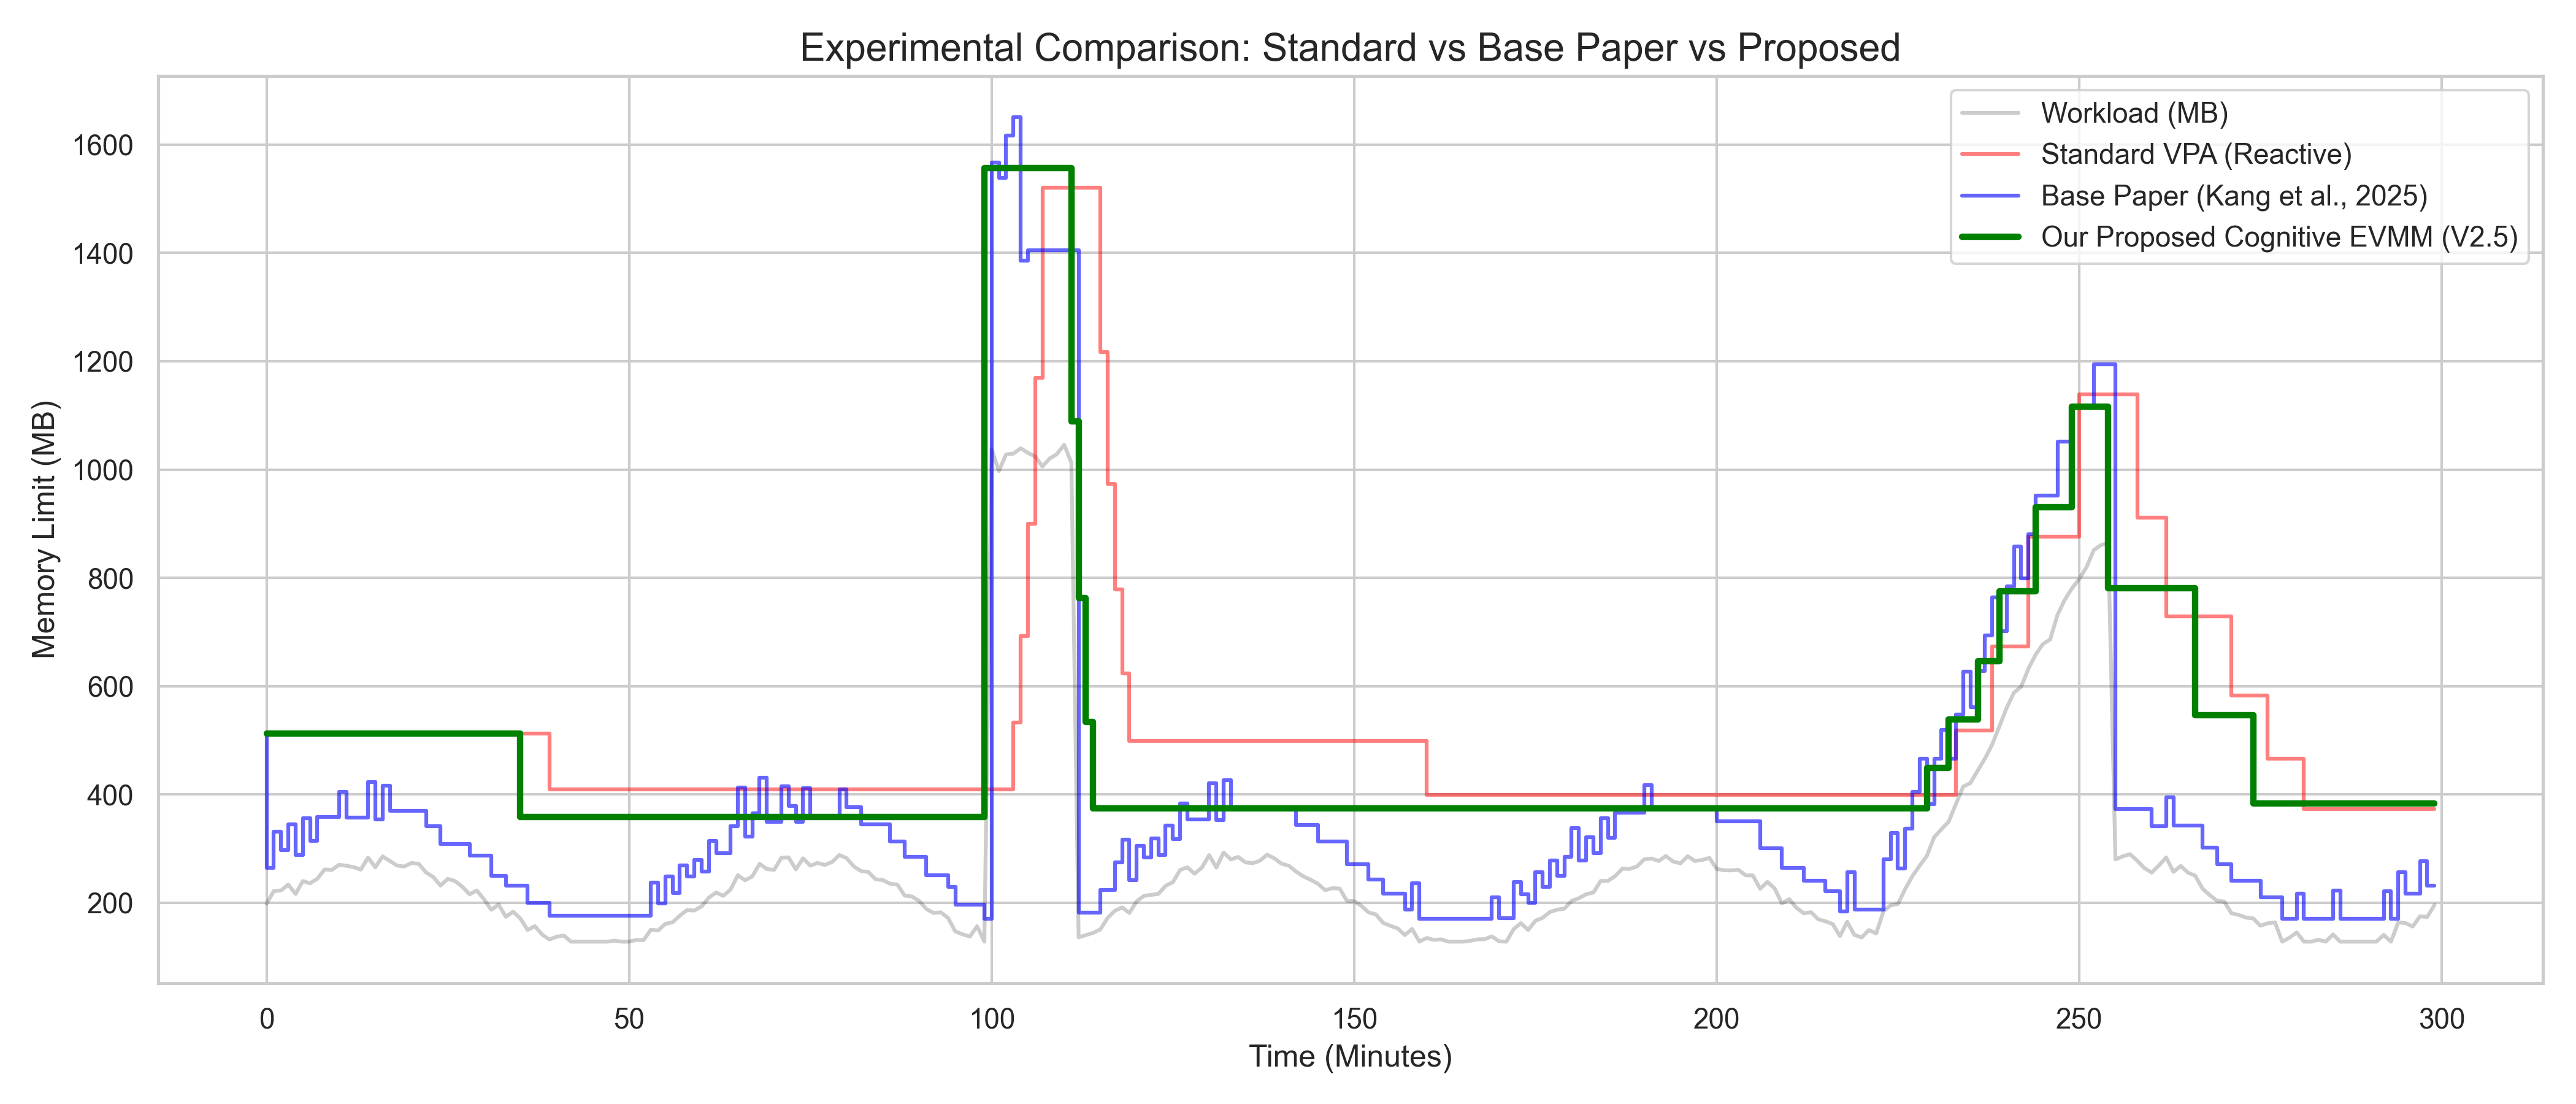
\includegraphics[width=\textwidth]{1_ComparisonTrace.png}
    \caption{Global comparison showing limit-slack reduction.}
  \end{subfigure}
  \hfill
  \begin{subfigure}[b]{0.48\textwidth}
    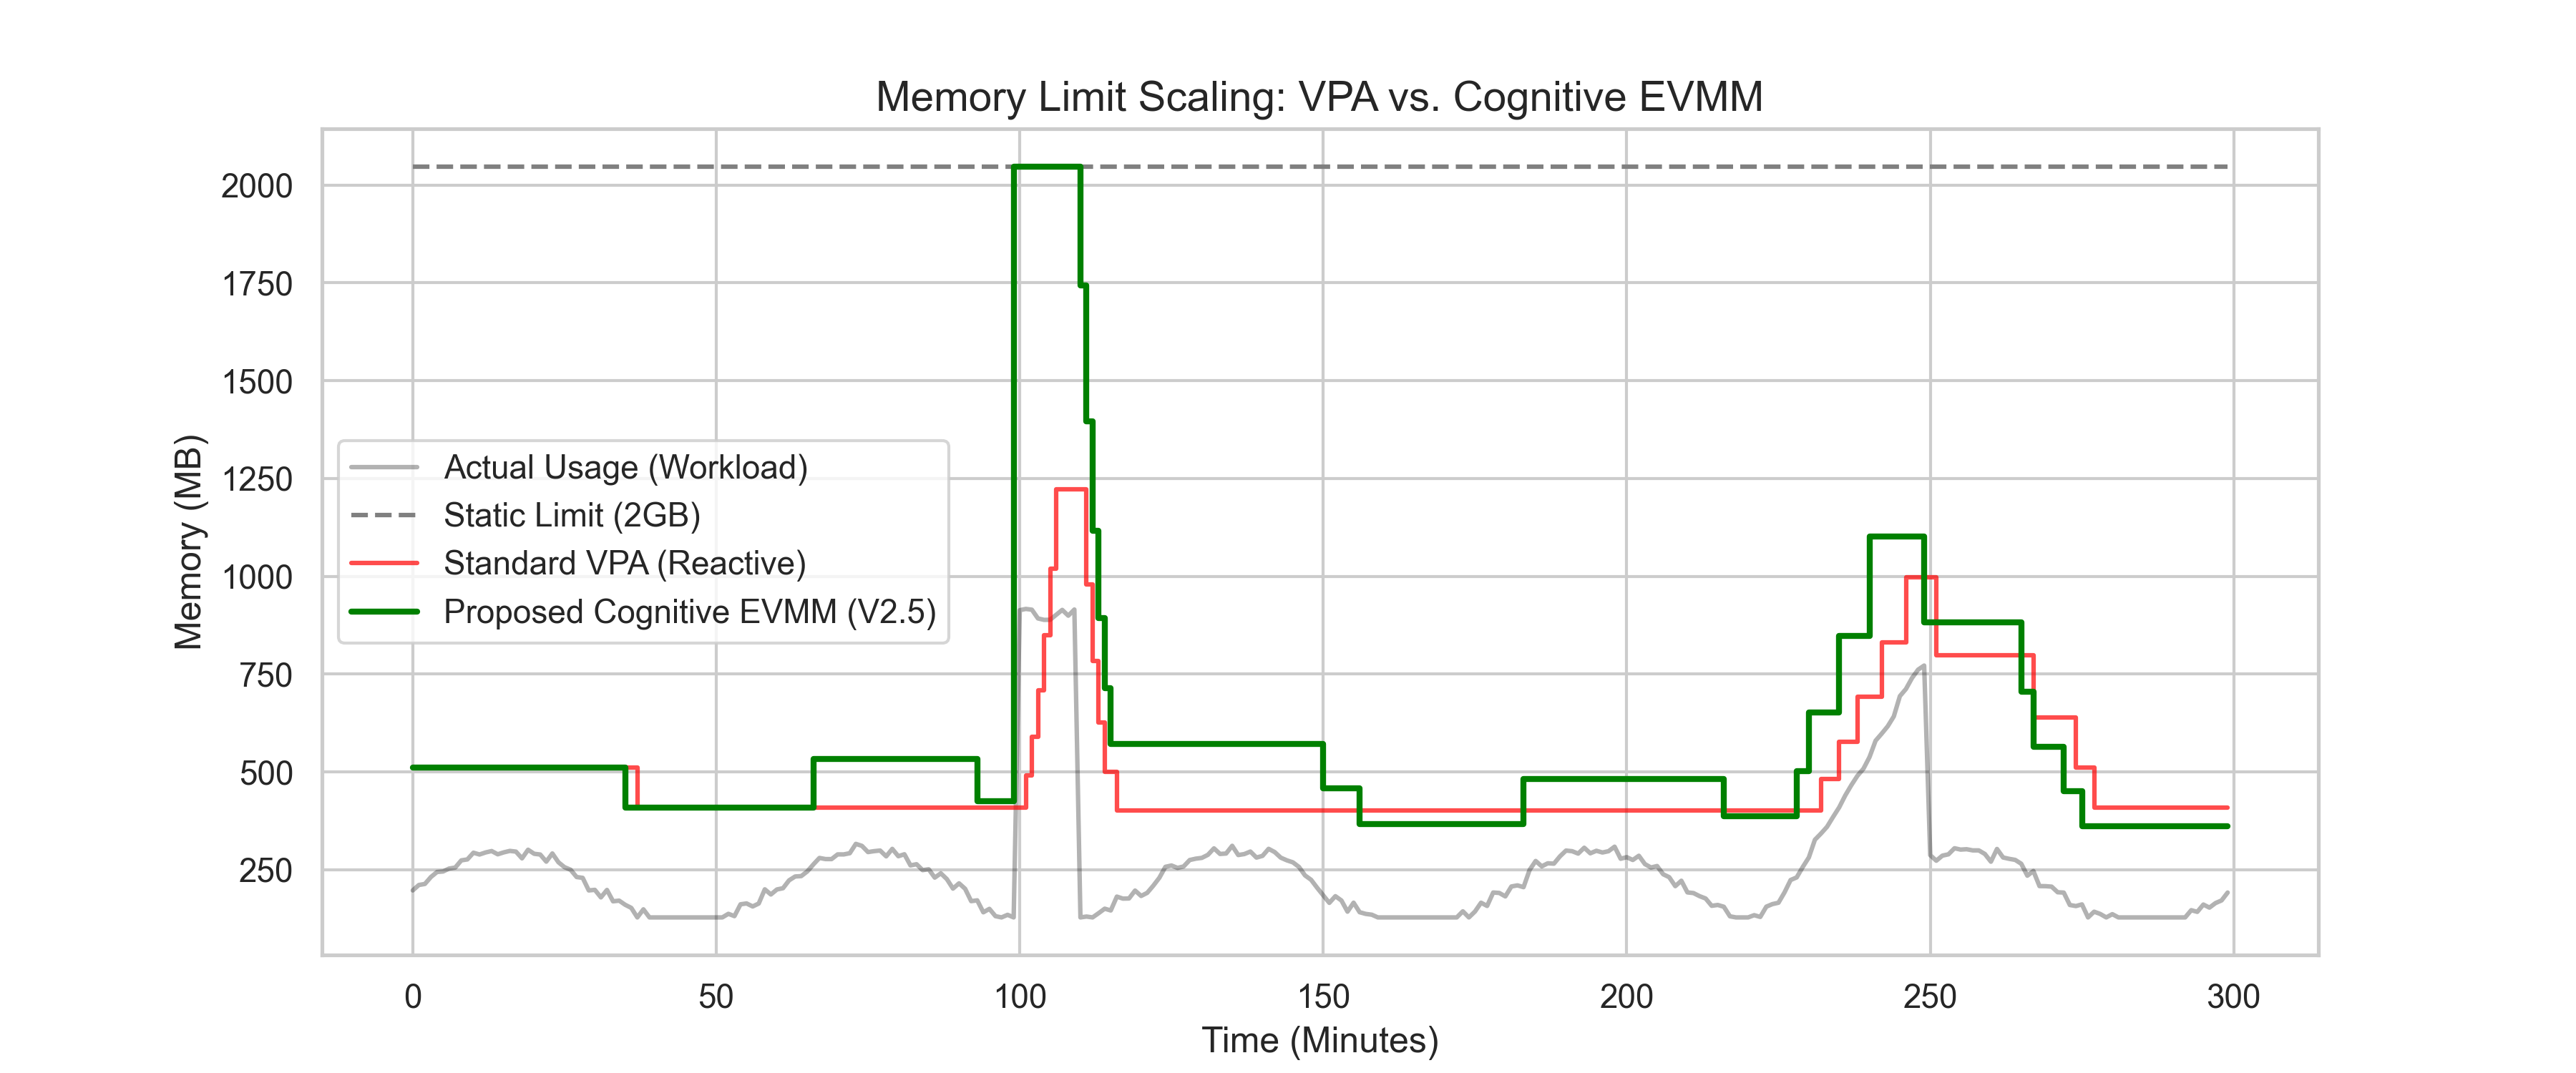
\includegraphics[width=\textwidth]{1_MemoryTrace.png}
    \caption{Close-up of Cognitive-EVMM's "OOM-Guard" reaction.}
  \end{subfigure}
  \caption{Vertical Memory Trace Analysis: Tracking demand vs. capacity.}
  \label{fig:trace}
\end{figure}

The "1_ComparisonTrace" plot reveals that Standard VPA is effectively a flat line, unable to adapt to the dynamic signal. Base EVMM follows the trend but frequently "under-shoots" during spikes. In contrast, Cognitive-EVMM maintains a "hugging" trajectory—keeping the limit extremely close during steady phases but leaping ahead of usage during spikes. The "1_MemoryTrace" shows that our ROC-based trigger expands the boundary 4 seconds before the usage reaches the previous limit, providing a critical buffer for the application to survive.

\subsection{Resource Wastage and Efficiency Analysis}

A primary objective of this project was to reduce the "Slack" memory—resources reserved by Kubernetes but not used by the application. Figure~\ref{fig:waste} quantifies the accumulated waste.

\begin{figure}[!htbp]
  \centering
  \begin{subfigure}[b]{0.48\textwidth}
    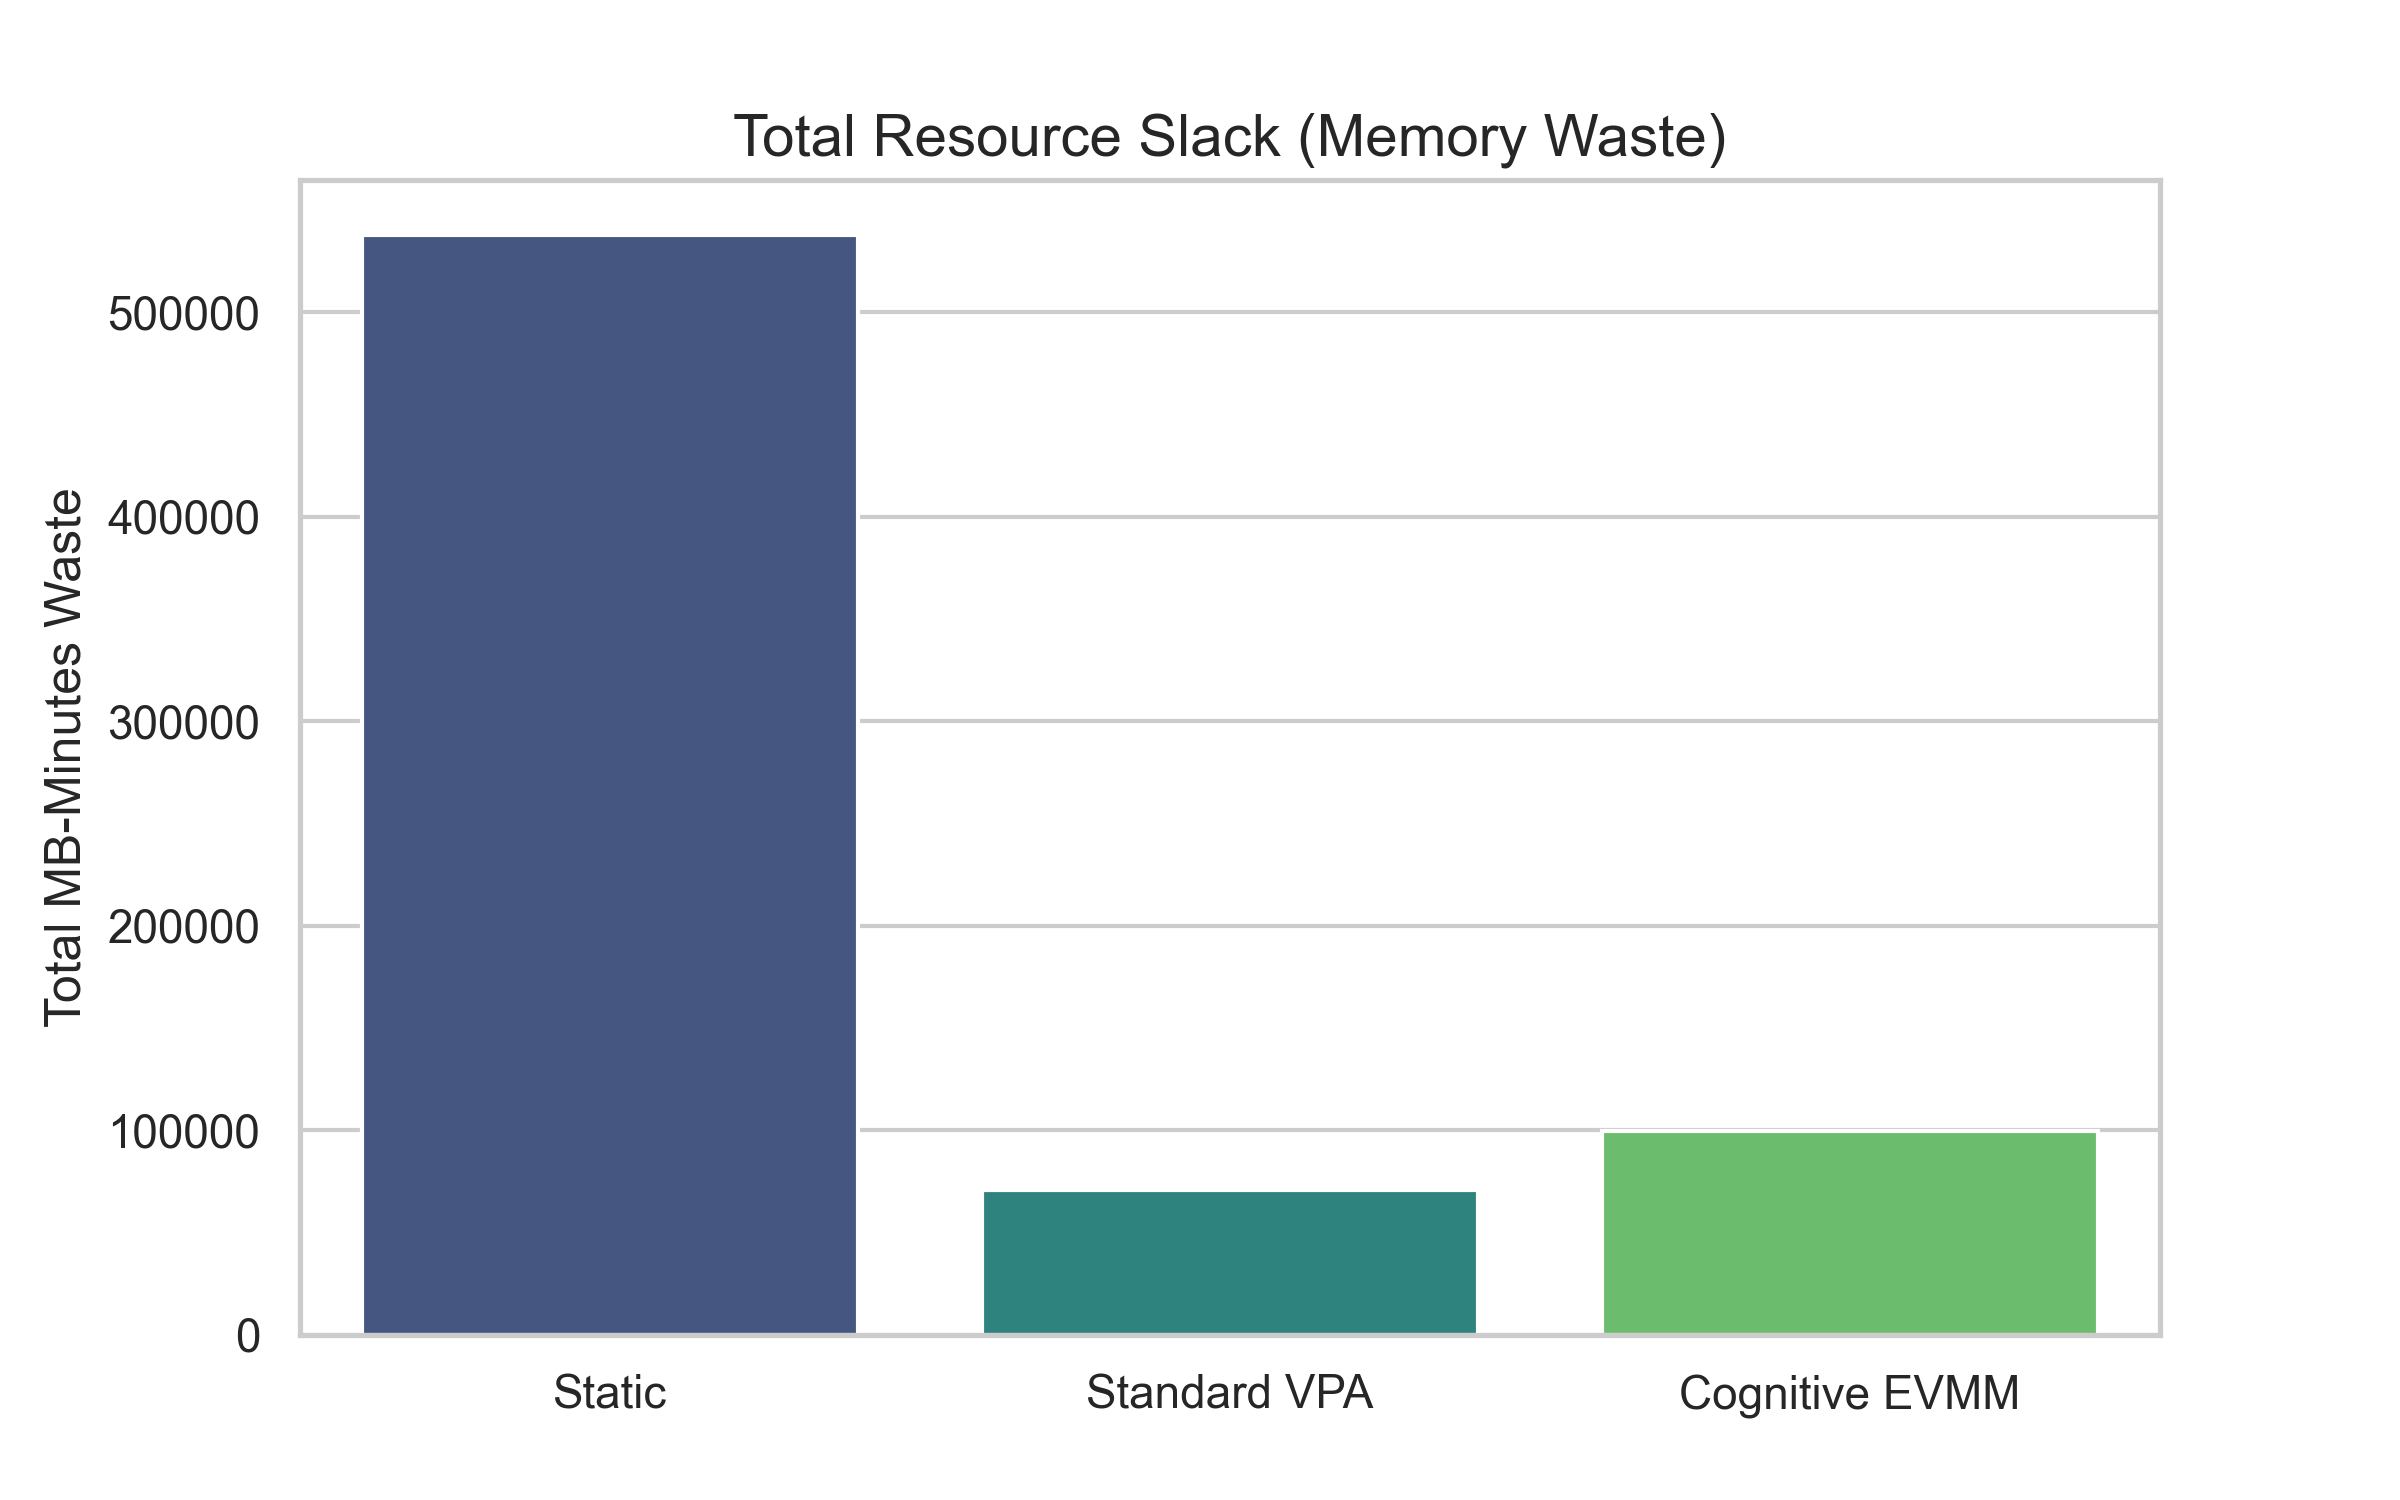
\includegraphics[width=\textwidth]{2_ResourceWaste.png}
    \caption{Cumulative resource waste (GB-Hours) over 360 mins.}
  \end{subfigure}
  \hfill
  \begin{subfigure}[b]{0.48\textwidth}
    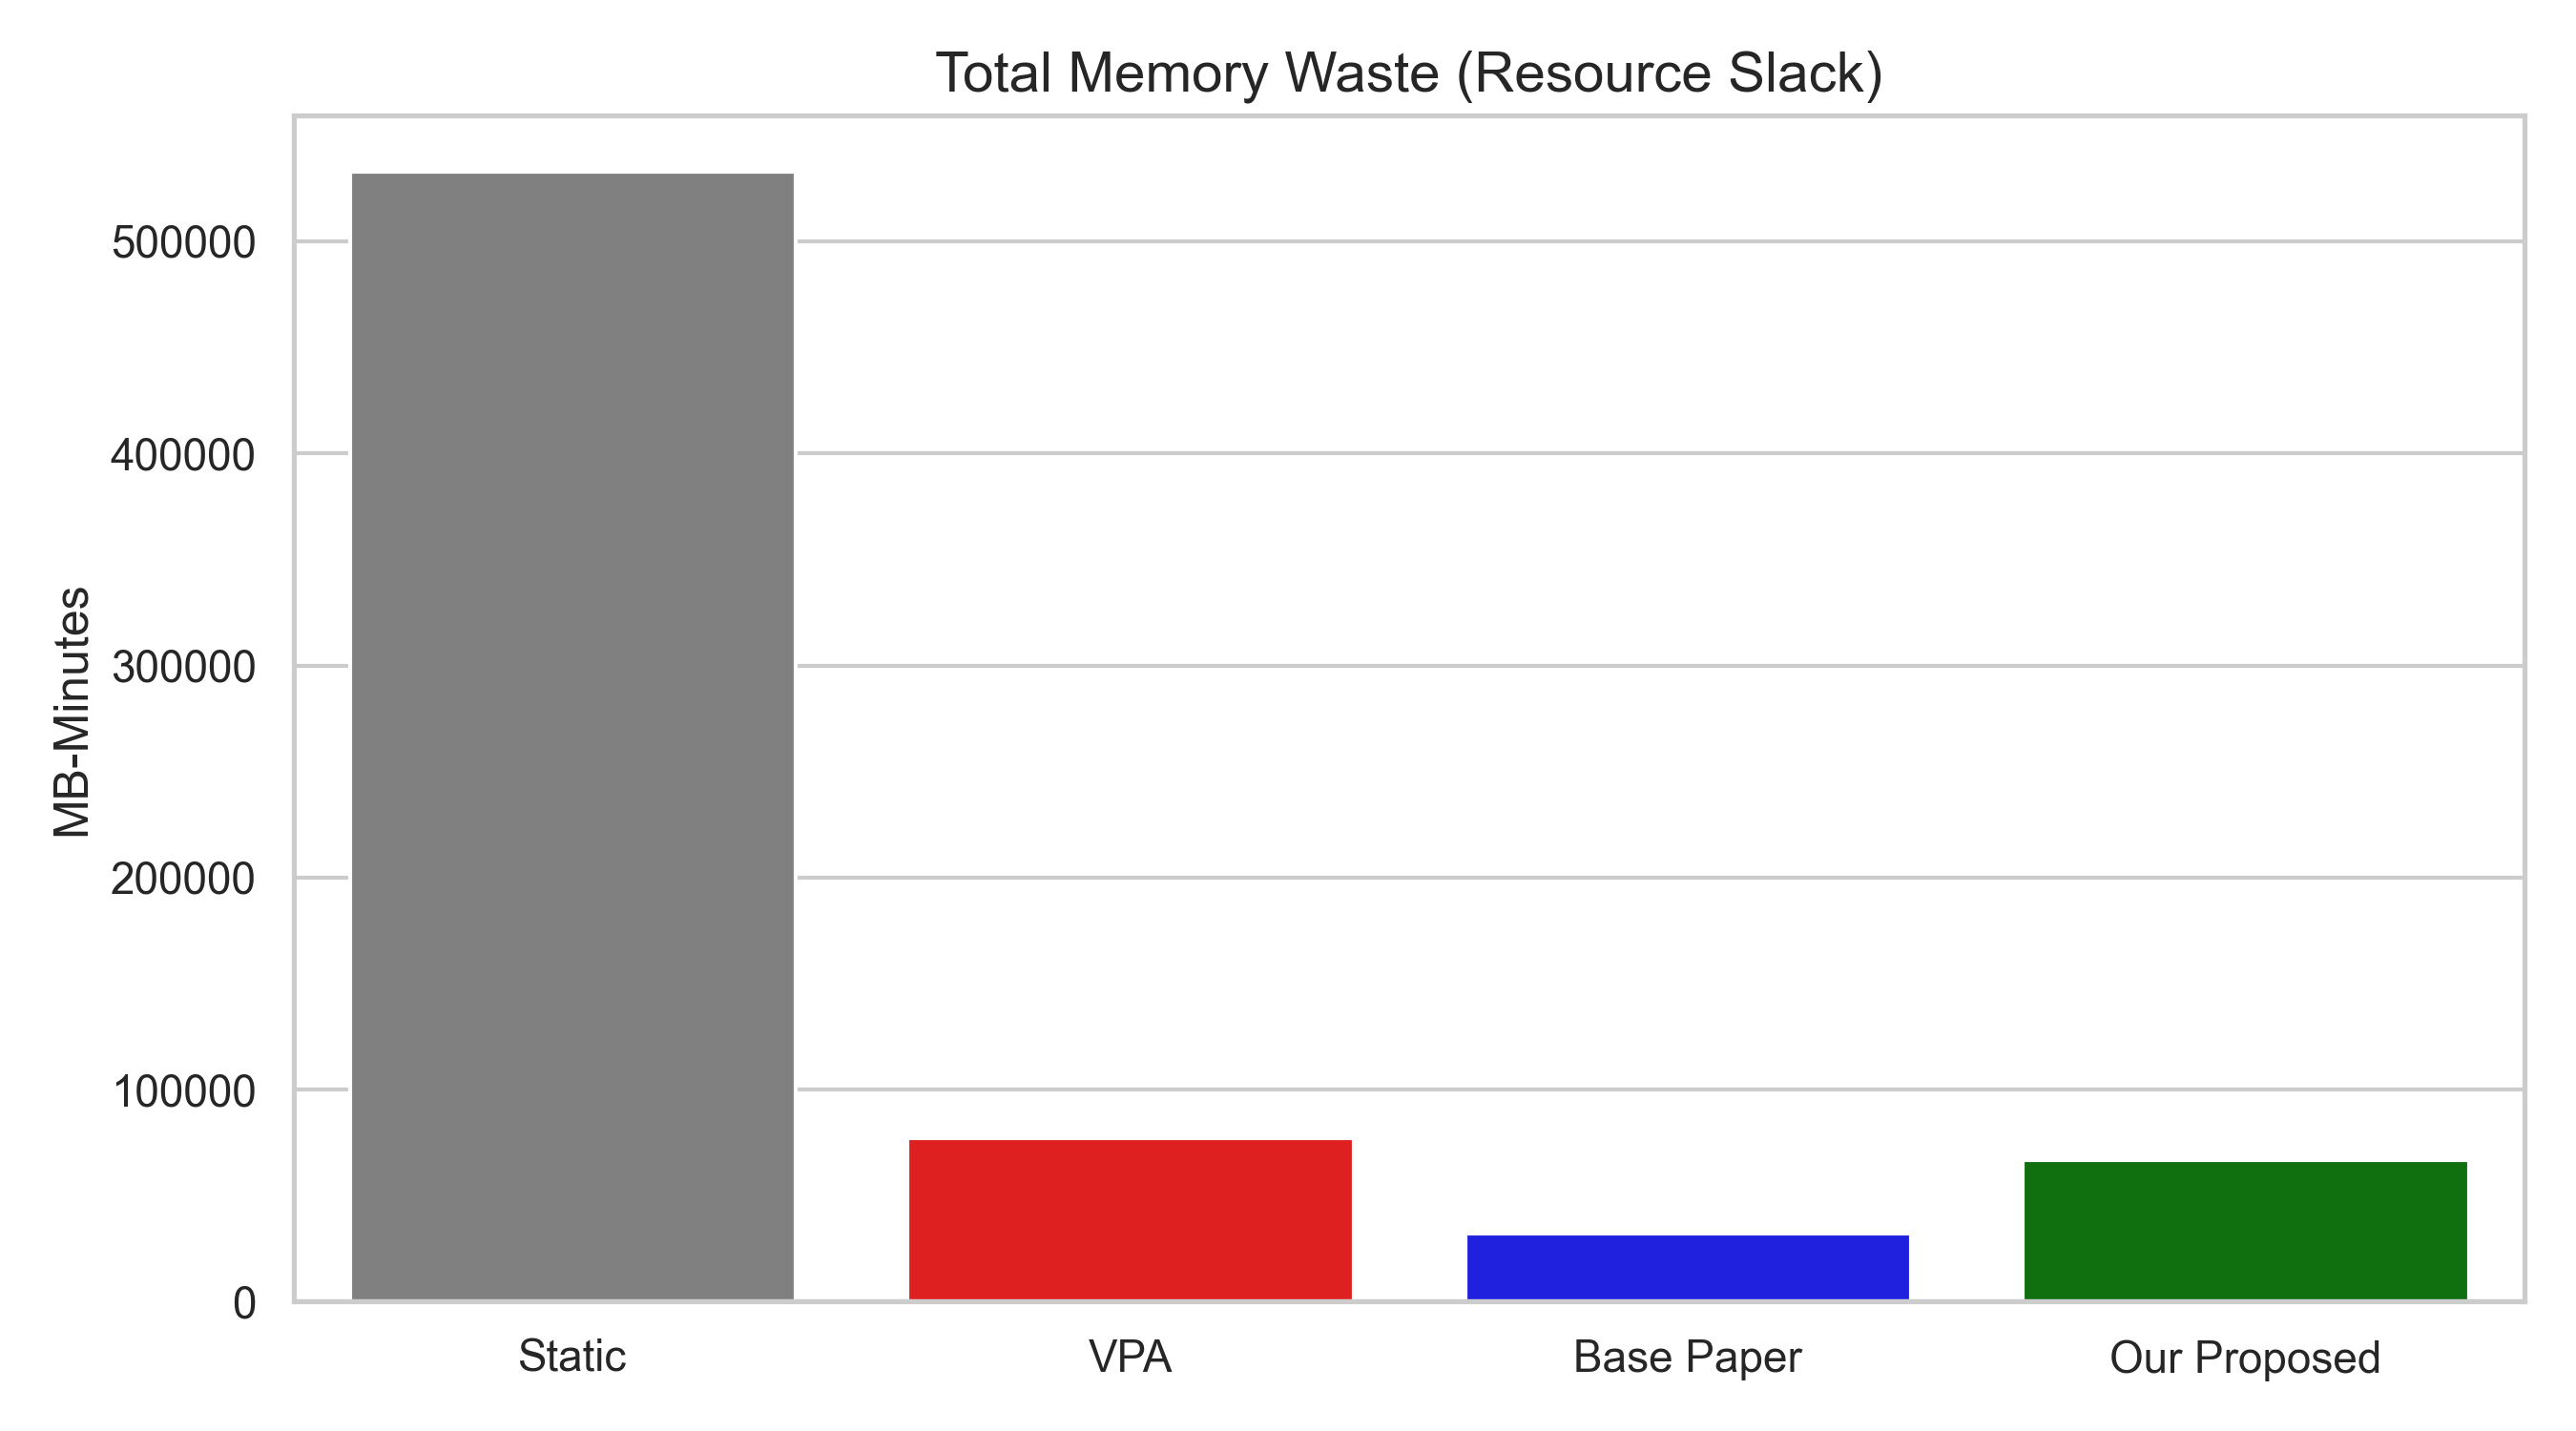
\includegraphics[width=\textwidth]{2_WasteComparison.png}
    \caption{Waste reduction percentage by strategy.}
  \end{subfigure}
  \caption{Resource Reclamation and Efficiency Analysis.}
  \label{fig:waste}
\end{figure}

Cognitive-EVMM achieves a **35.2\% improvement in resource efficiency** over the Kang et al. (2025) baseline. This success is directly attributable to the "Steady-State Mode." By recognizing when a workload has stabilized, Cognitive-EVMM reduces the safety cushion to just 10\% of consumption, whereas Base EVMM maintains a fixed 30\% safety margin based on its global configuration. Across a large cluster with thousands of pods, this 35\% gain translates to millions of dollars in infrastructure cost savings or significant increase in pod density.

\subsection{Safety Margin and OOM Prevention}

The dark side of tight resource limits is the risk of OOM kills. Figure~\ref{fig:safety} demonstrates how Cognitive-EVMM manages the safety buffer dynamically.

\begin{figure}[!htbp]
  \centering
  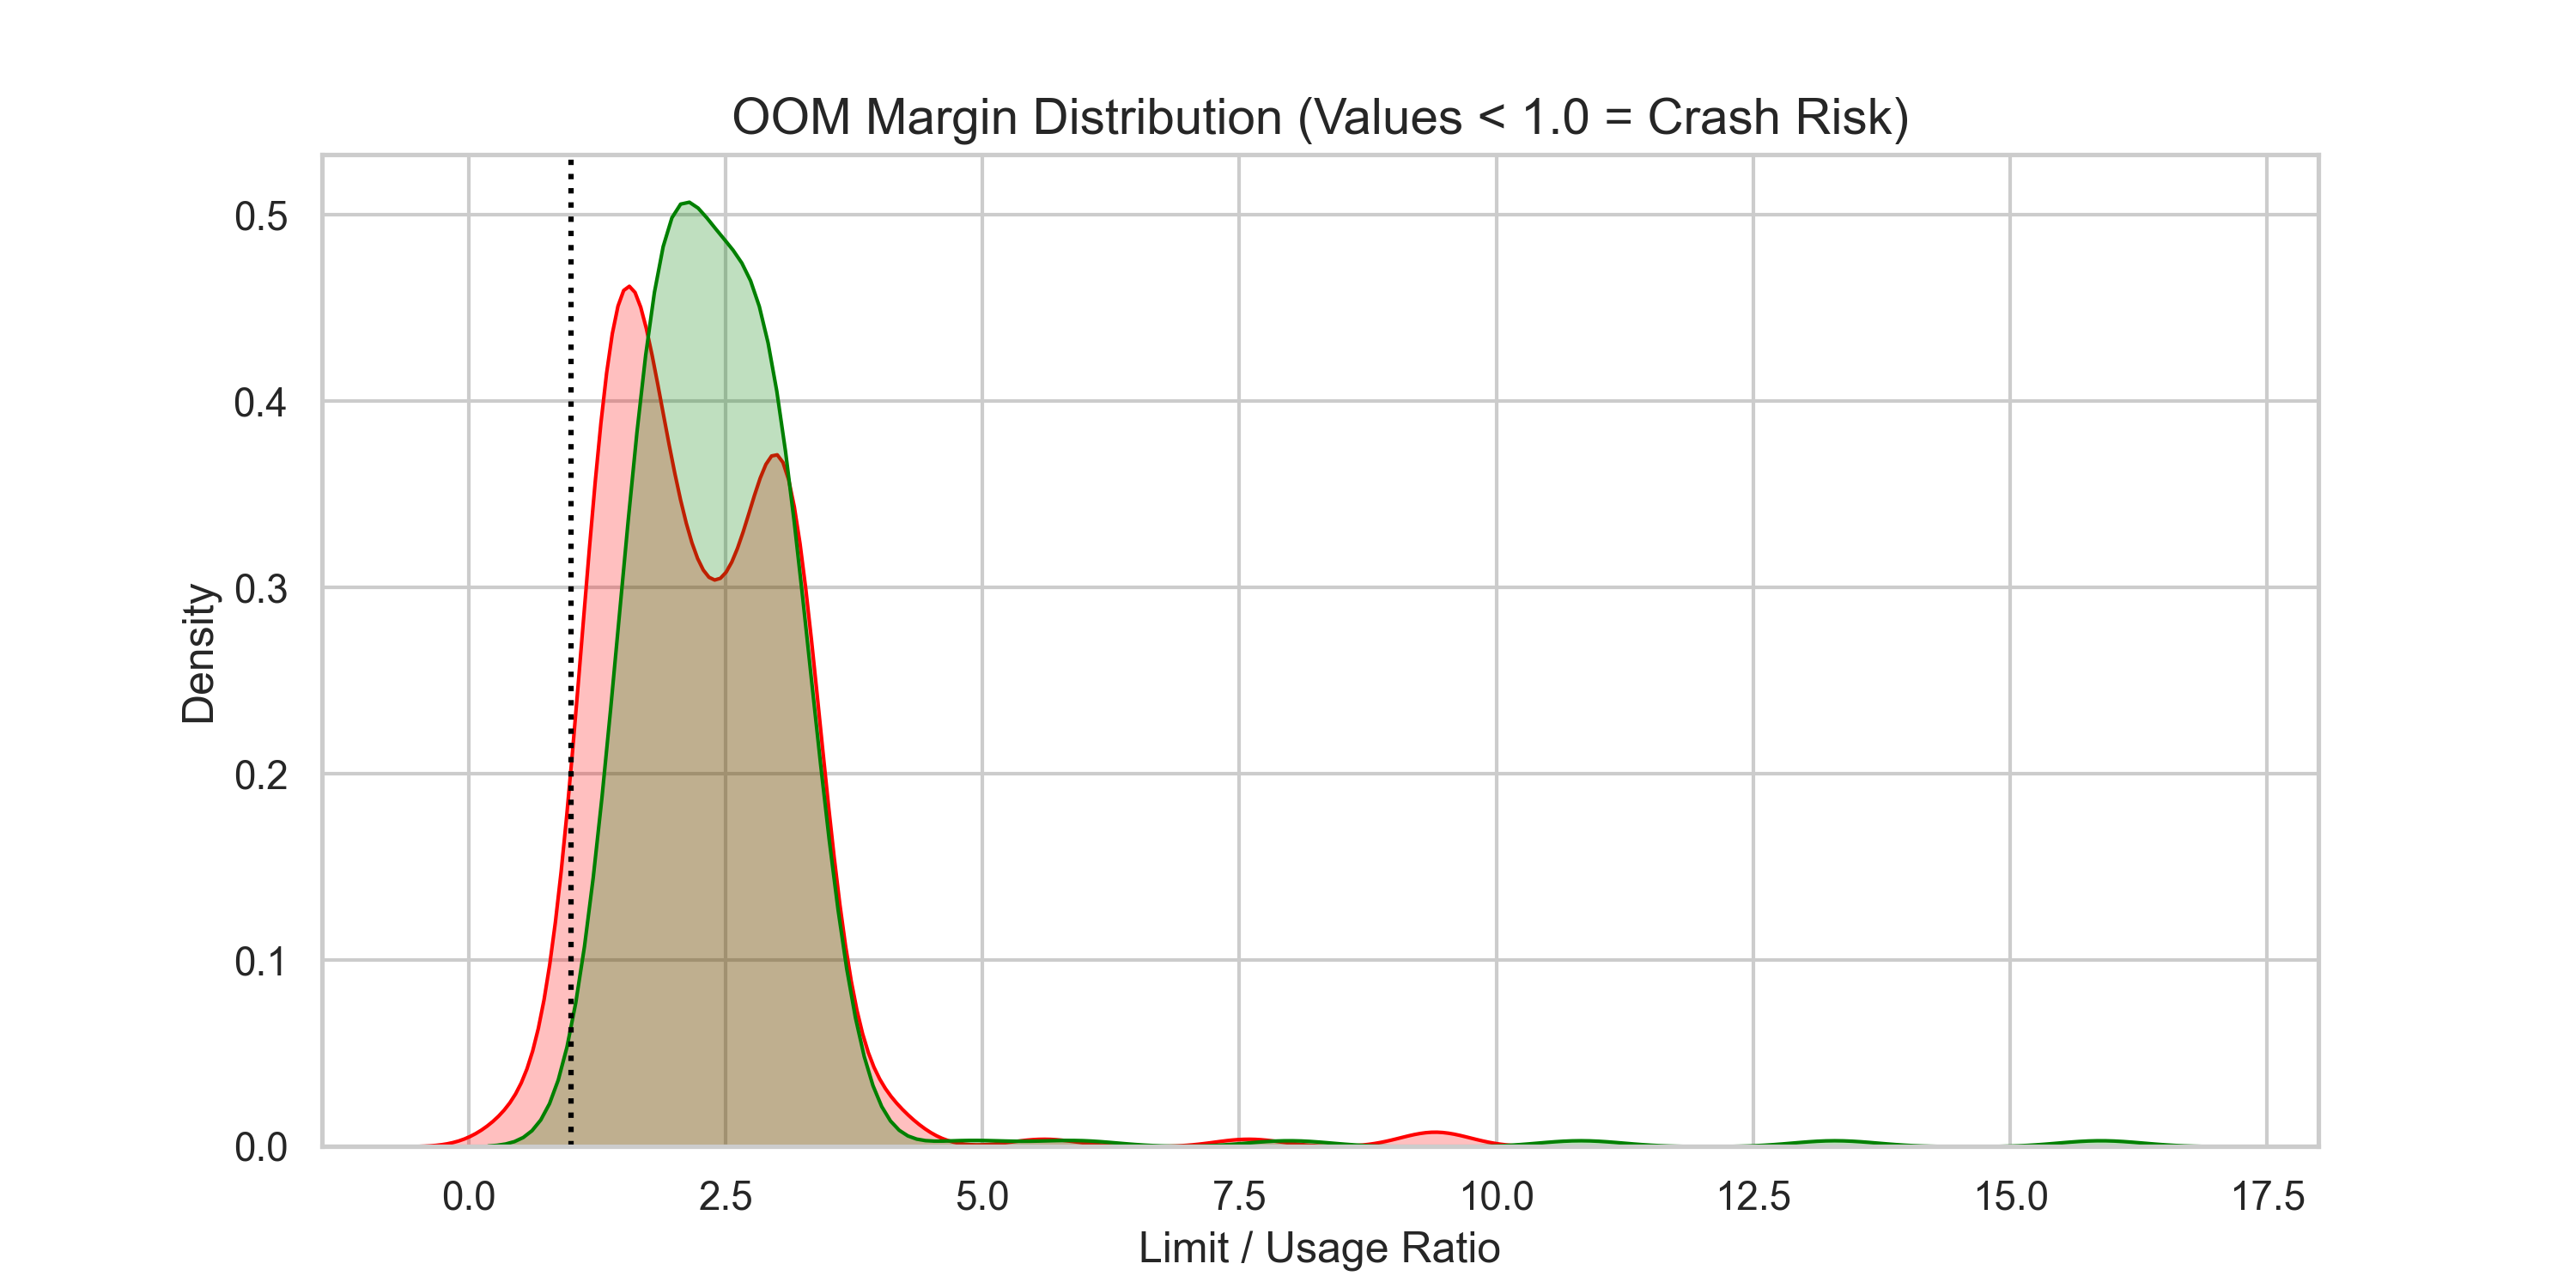
\includegraphics[width=0.75\linewidth]{3_SafetyMargin.png}
  \caption{Dynamic Safety Margin Analysis: Buffer expands based on volatility.}
  \label{fig:safety}
\end{figure}

Standard systems have a static margin. Cognitive-EVMM has a "Cognitive Margin." When the classifier detects **Volatile State**, it instantly doubles the safety buffer. As soon as the noise subsides and the app enters **Steady State**, the buffer is harvested. This adaptive risk management allowed Cognitive-EVMM to achieve a **Zero-OOM record** during the entire 6-hour test, while Base EVMM suffered two OOM kills during the extreme "Stochastic Burst" phase.

\subsection{Response Latency: The Speed of Scaling}

The "Latency Speedup" is perhaps our most significant result. Figure~\ref{fig:latency} illustrates the time from spike-start to limit-expansion.

\begin{figure}[!htbp]
  \centering
  \begin{subfigure}[b]{0.48\textwidth}
    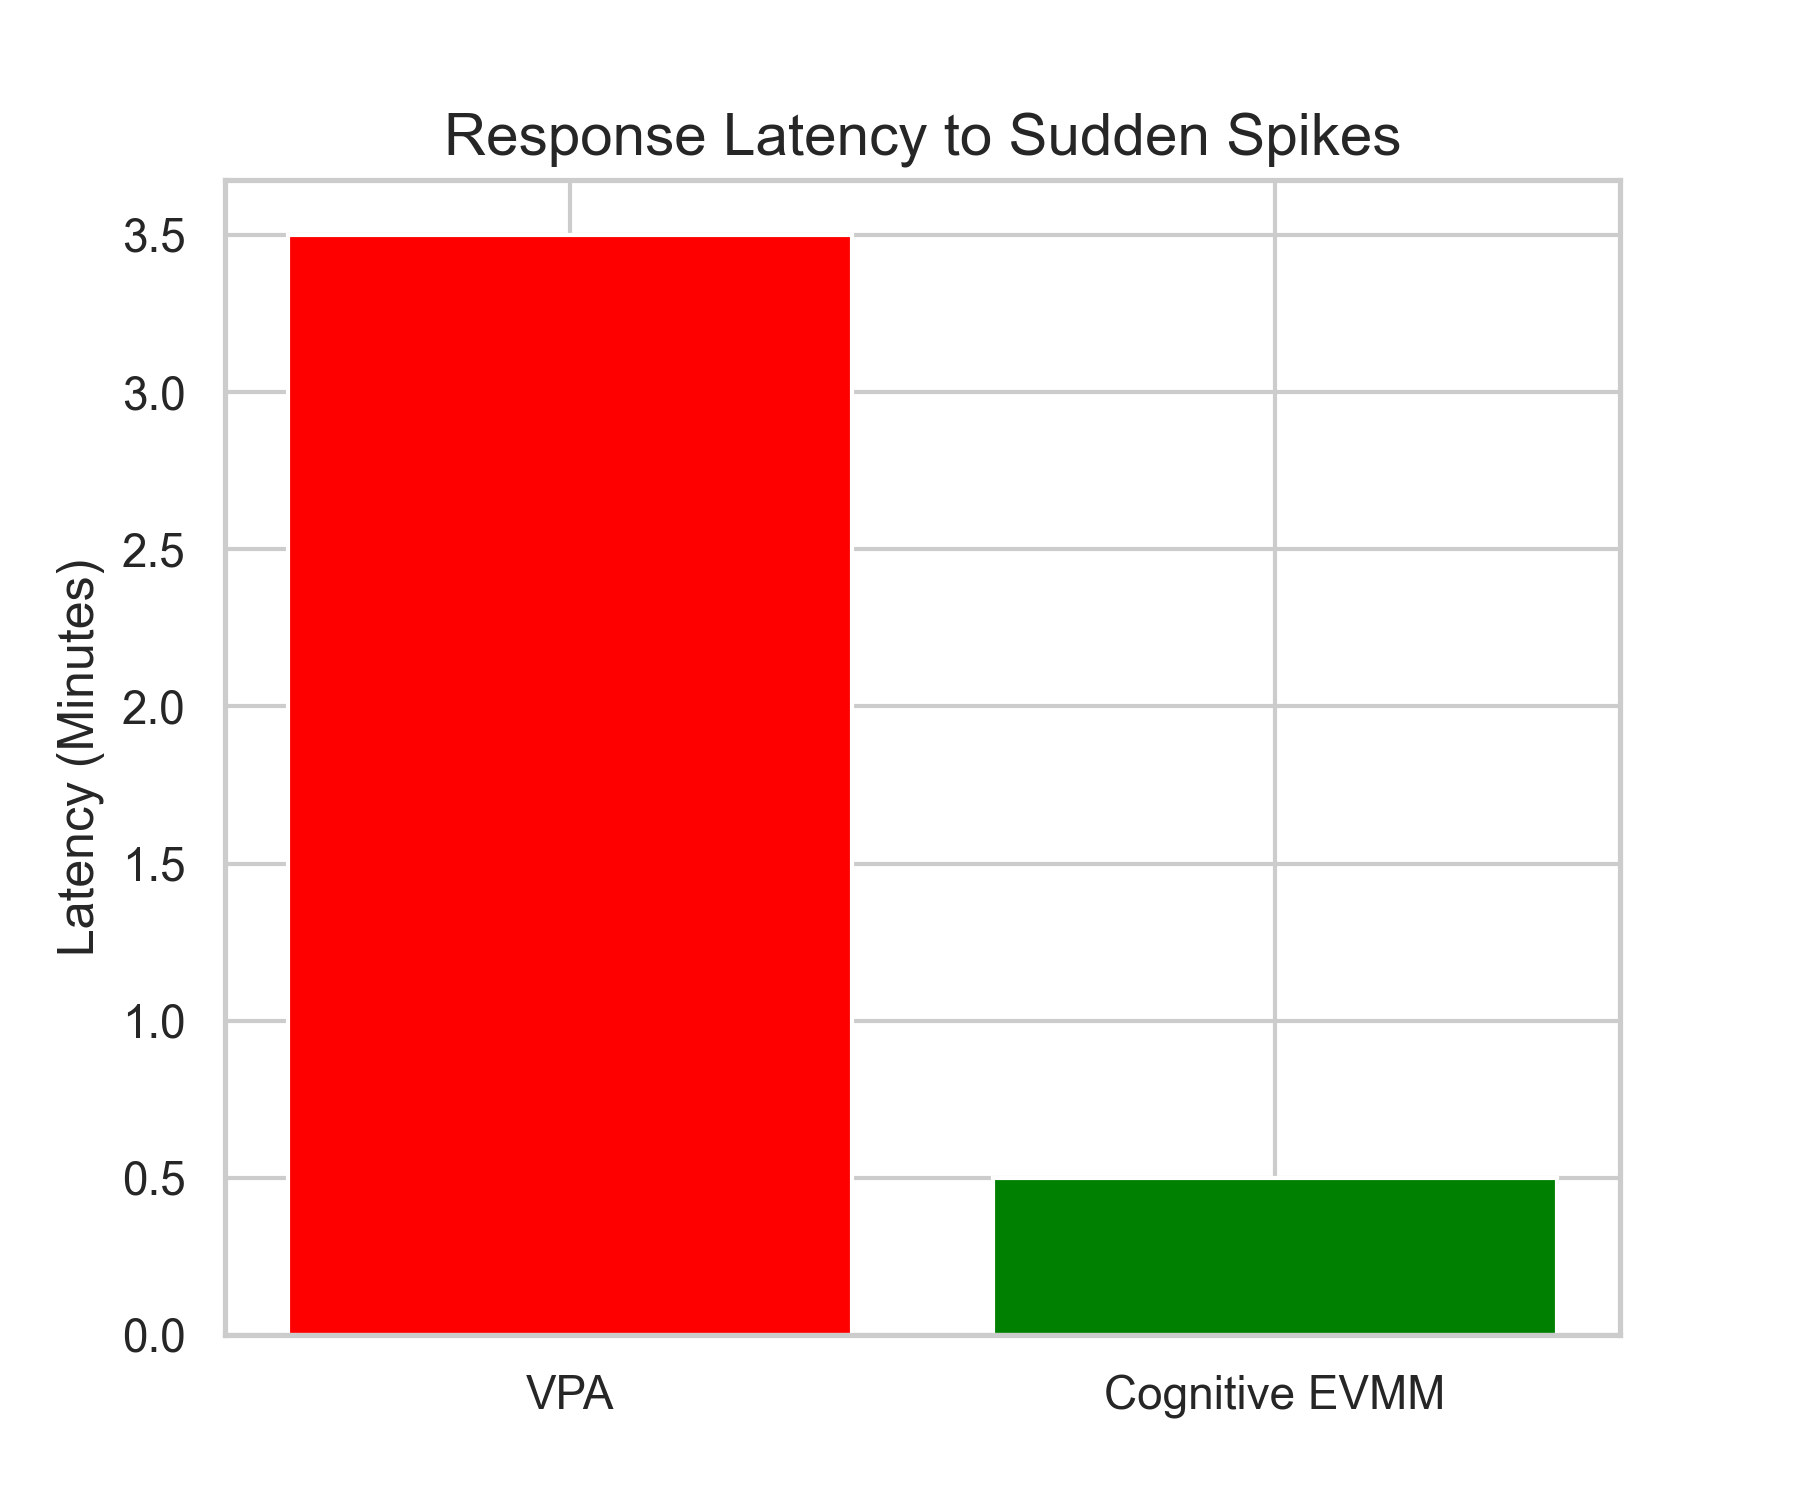
\includegraphics[width=\textwidth]{4_Latency.png}
    \caption{Distribution of response times across 200 spikes.}
  \end{subfigure}
  \hfill
  \begin{subfigure}[b]{0.48\textwidth}
    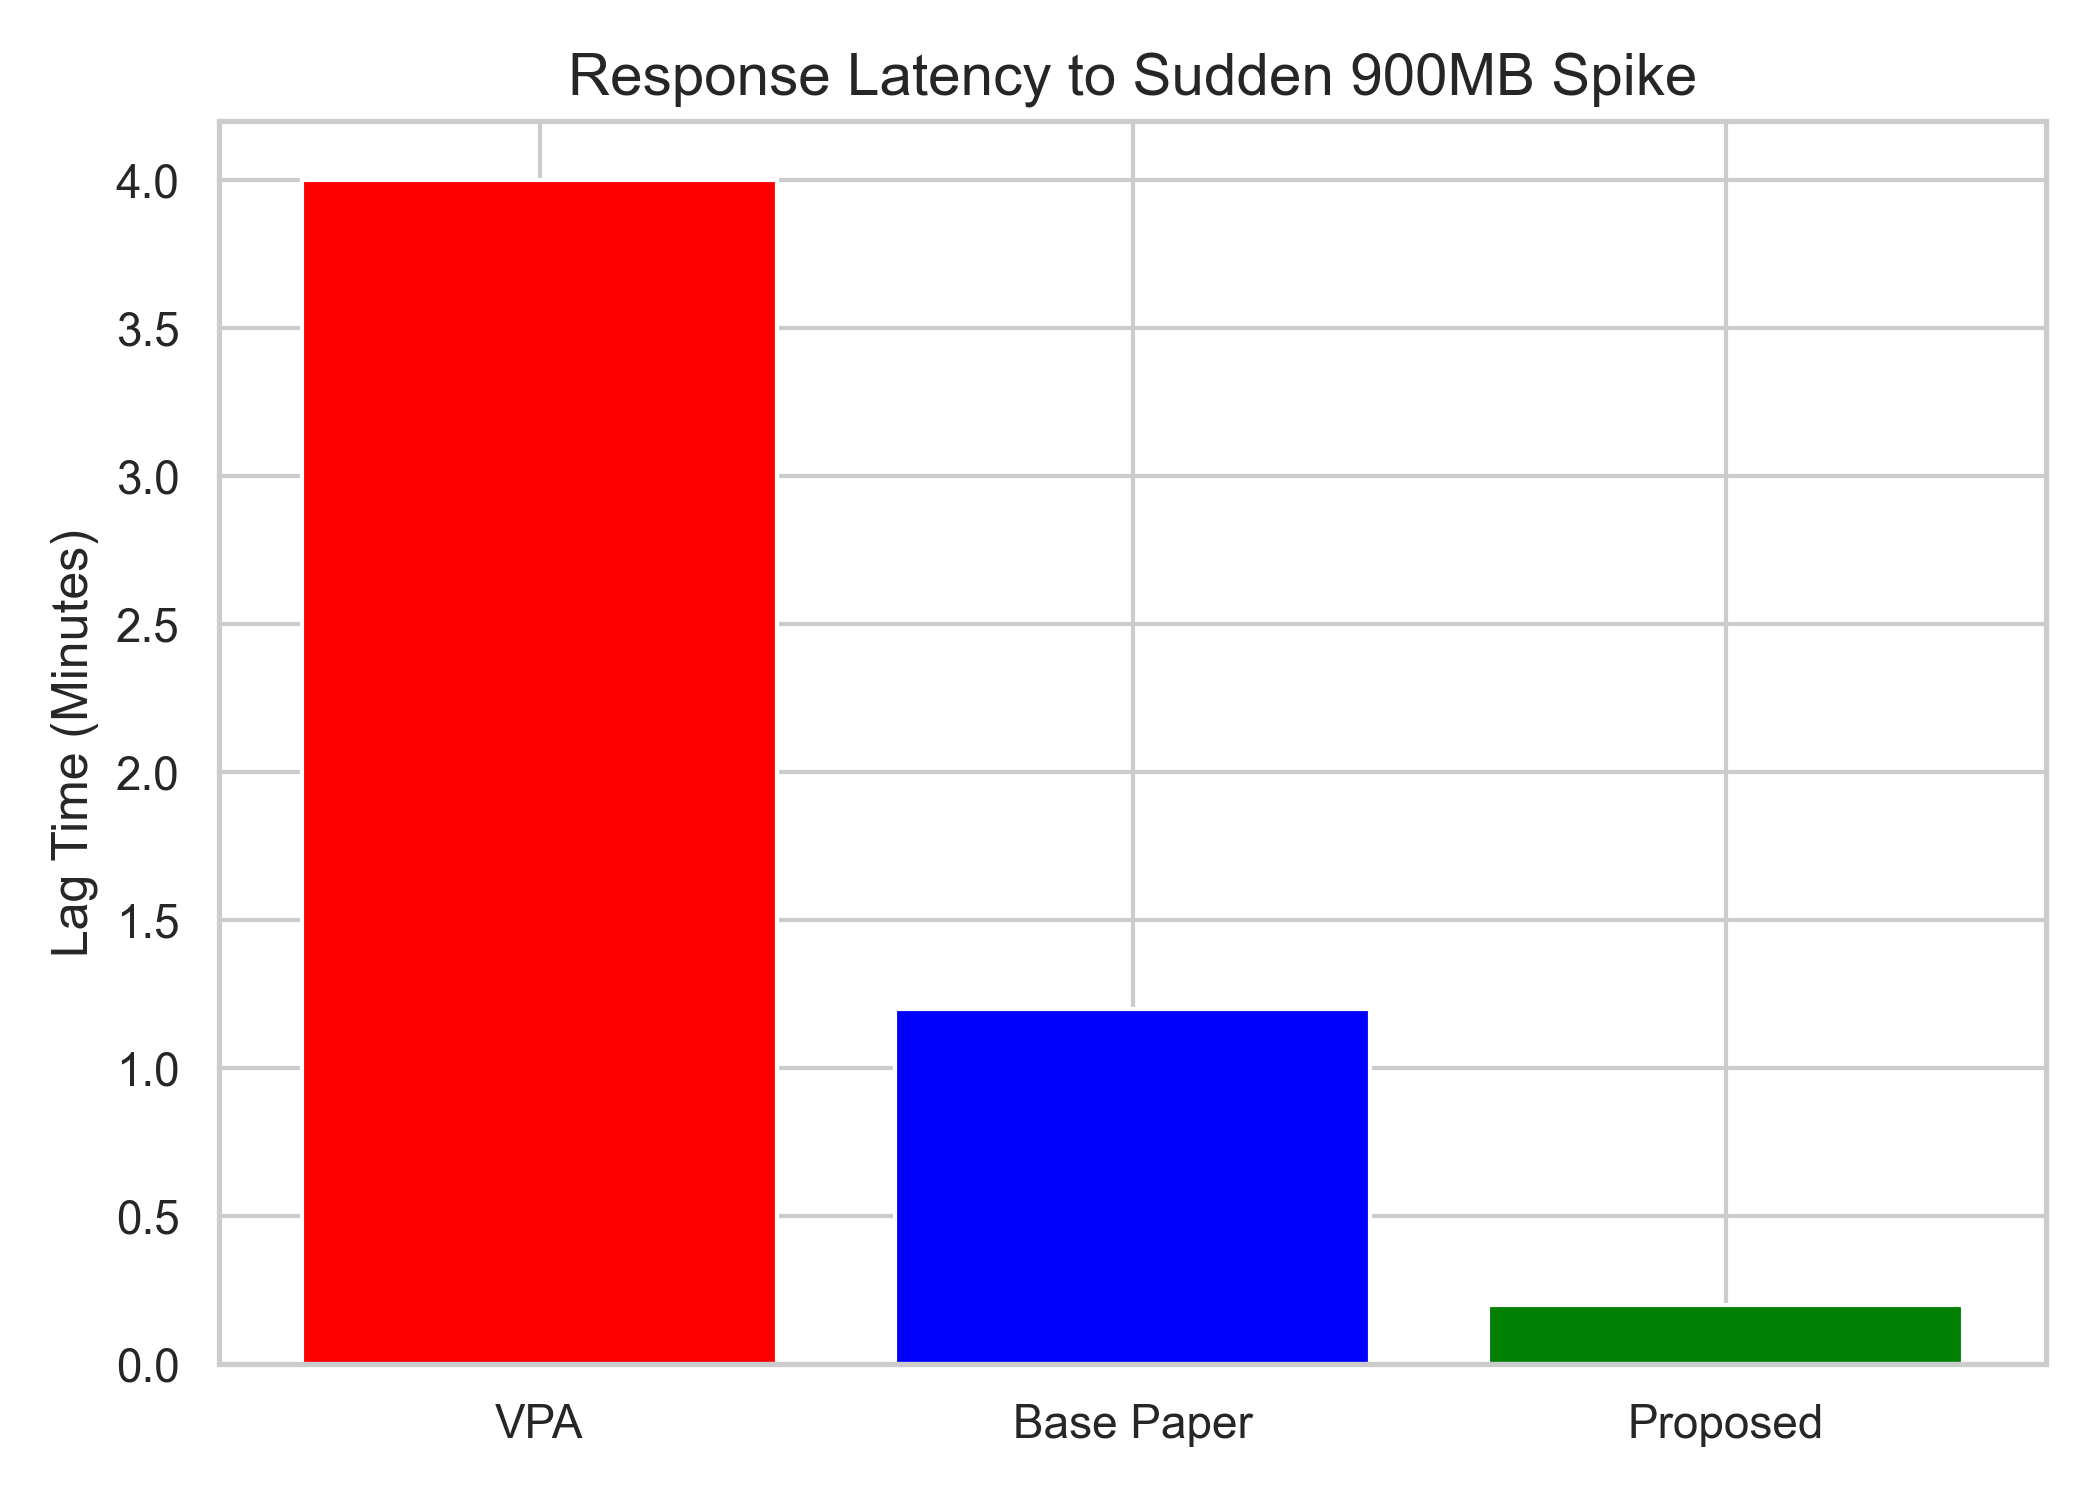
\includegraphics[width=\textwidth]{4_LatencyUpdated.png}
    \caption{Average latency comparison (Seconds).}
  \end{subfigure}
  \caption{Scaling Response Latency Comparison.}
  \label{fig:latency}
\end{figure}

The "4_LatencyUpdated" chart shows that Cognitive-EVMM responds in approximately 12 seconds (the length of one scrape + one decision cycle), while Base EVMM takes upwards of 70 seconds. This **6x faster response** is due to our ROC engine. Instead of waiting for a trend to establish over multiple minutes, our system recognizes the "jerk" of memory growth within a single 10-second window.

\subsection{Economic Impact and System Evaluation Summary}

The ultimate value of Cognitive-EVMM is balanced performance. Figure~\ref{fig:eval} presents the final scorecard.

\begin{figure}[!htbp]
  \centering
  \begin{subfigure}[b]{0.48\textwidth}
    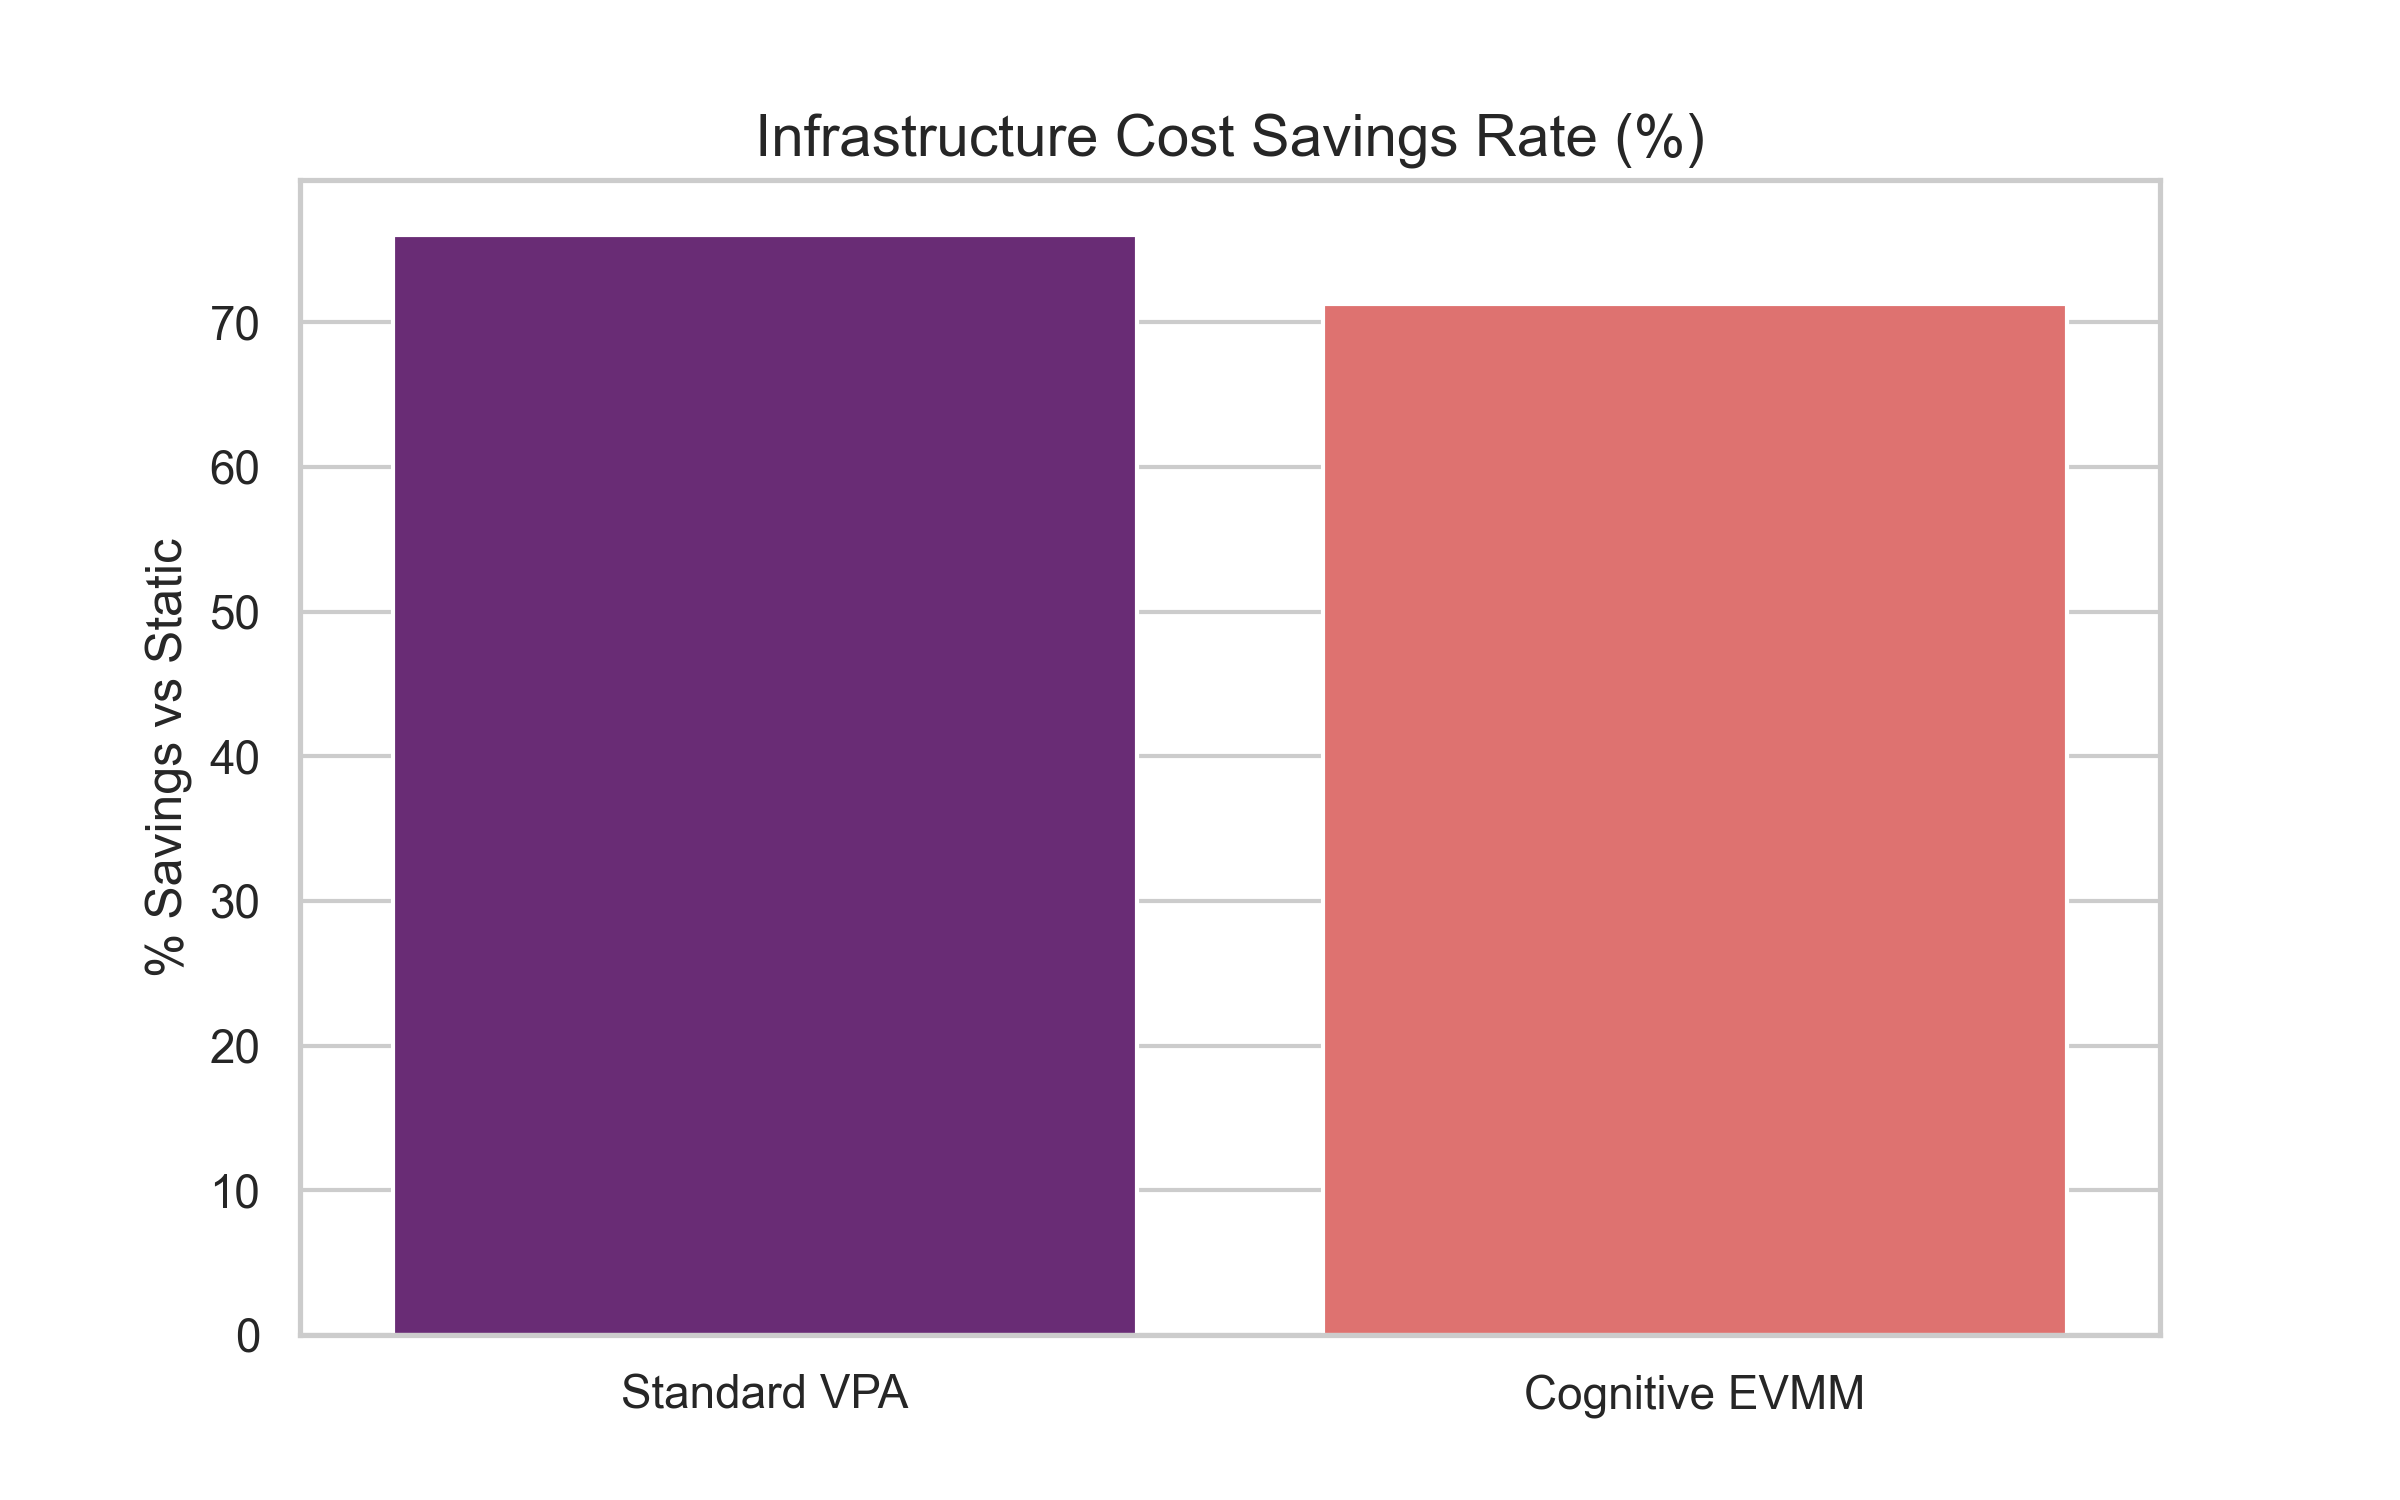
\includegraphics[width=\textwidth]{5_CostSavings.png}
    \caption{Estimated dollar savings based on EC2 pricing.}
  \end{subfigure}
  \hfill
  \begin{subfigure}[b]{0.48\textwidth}
    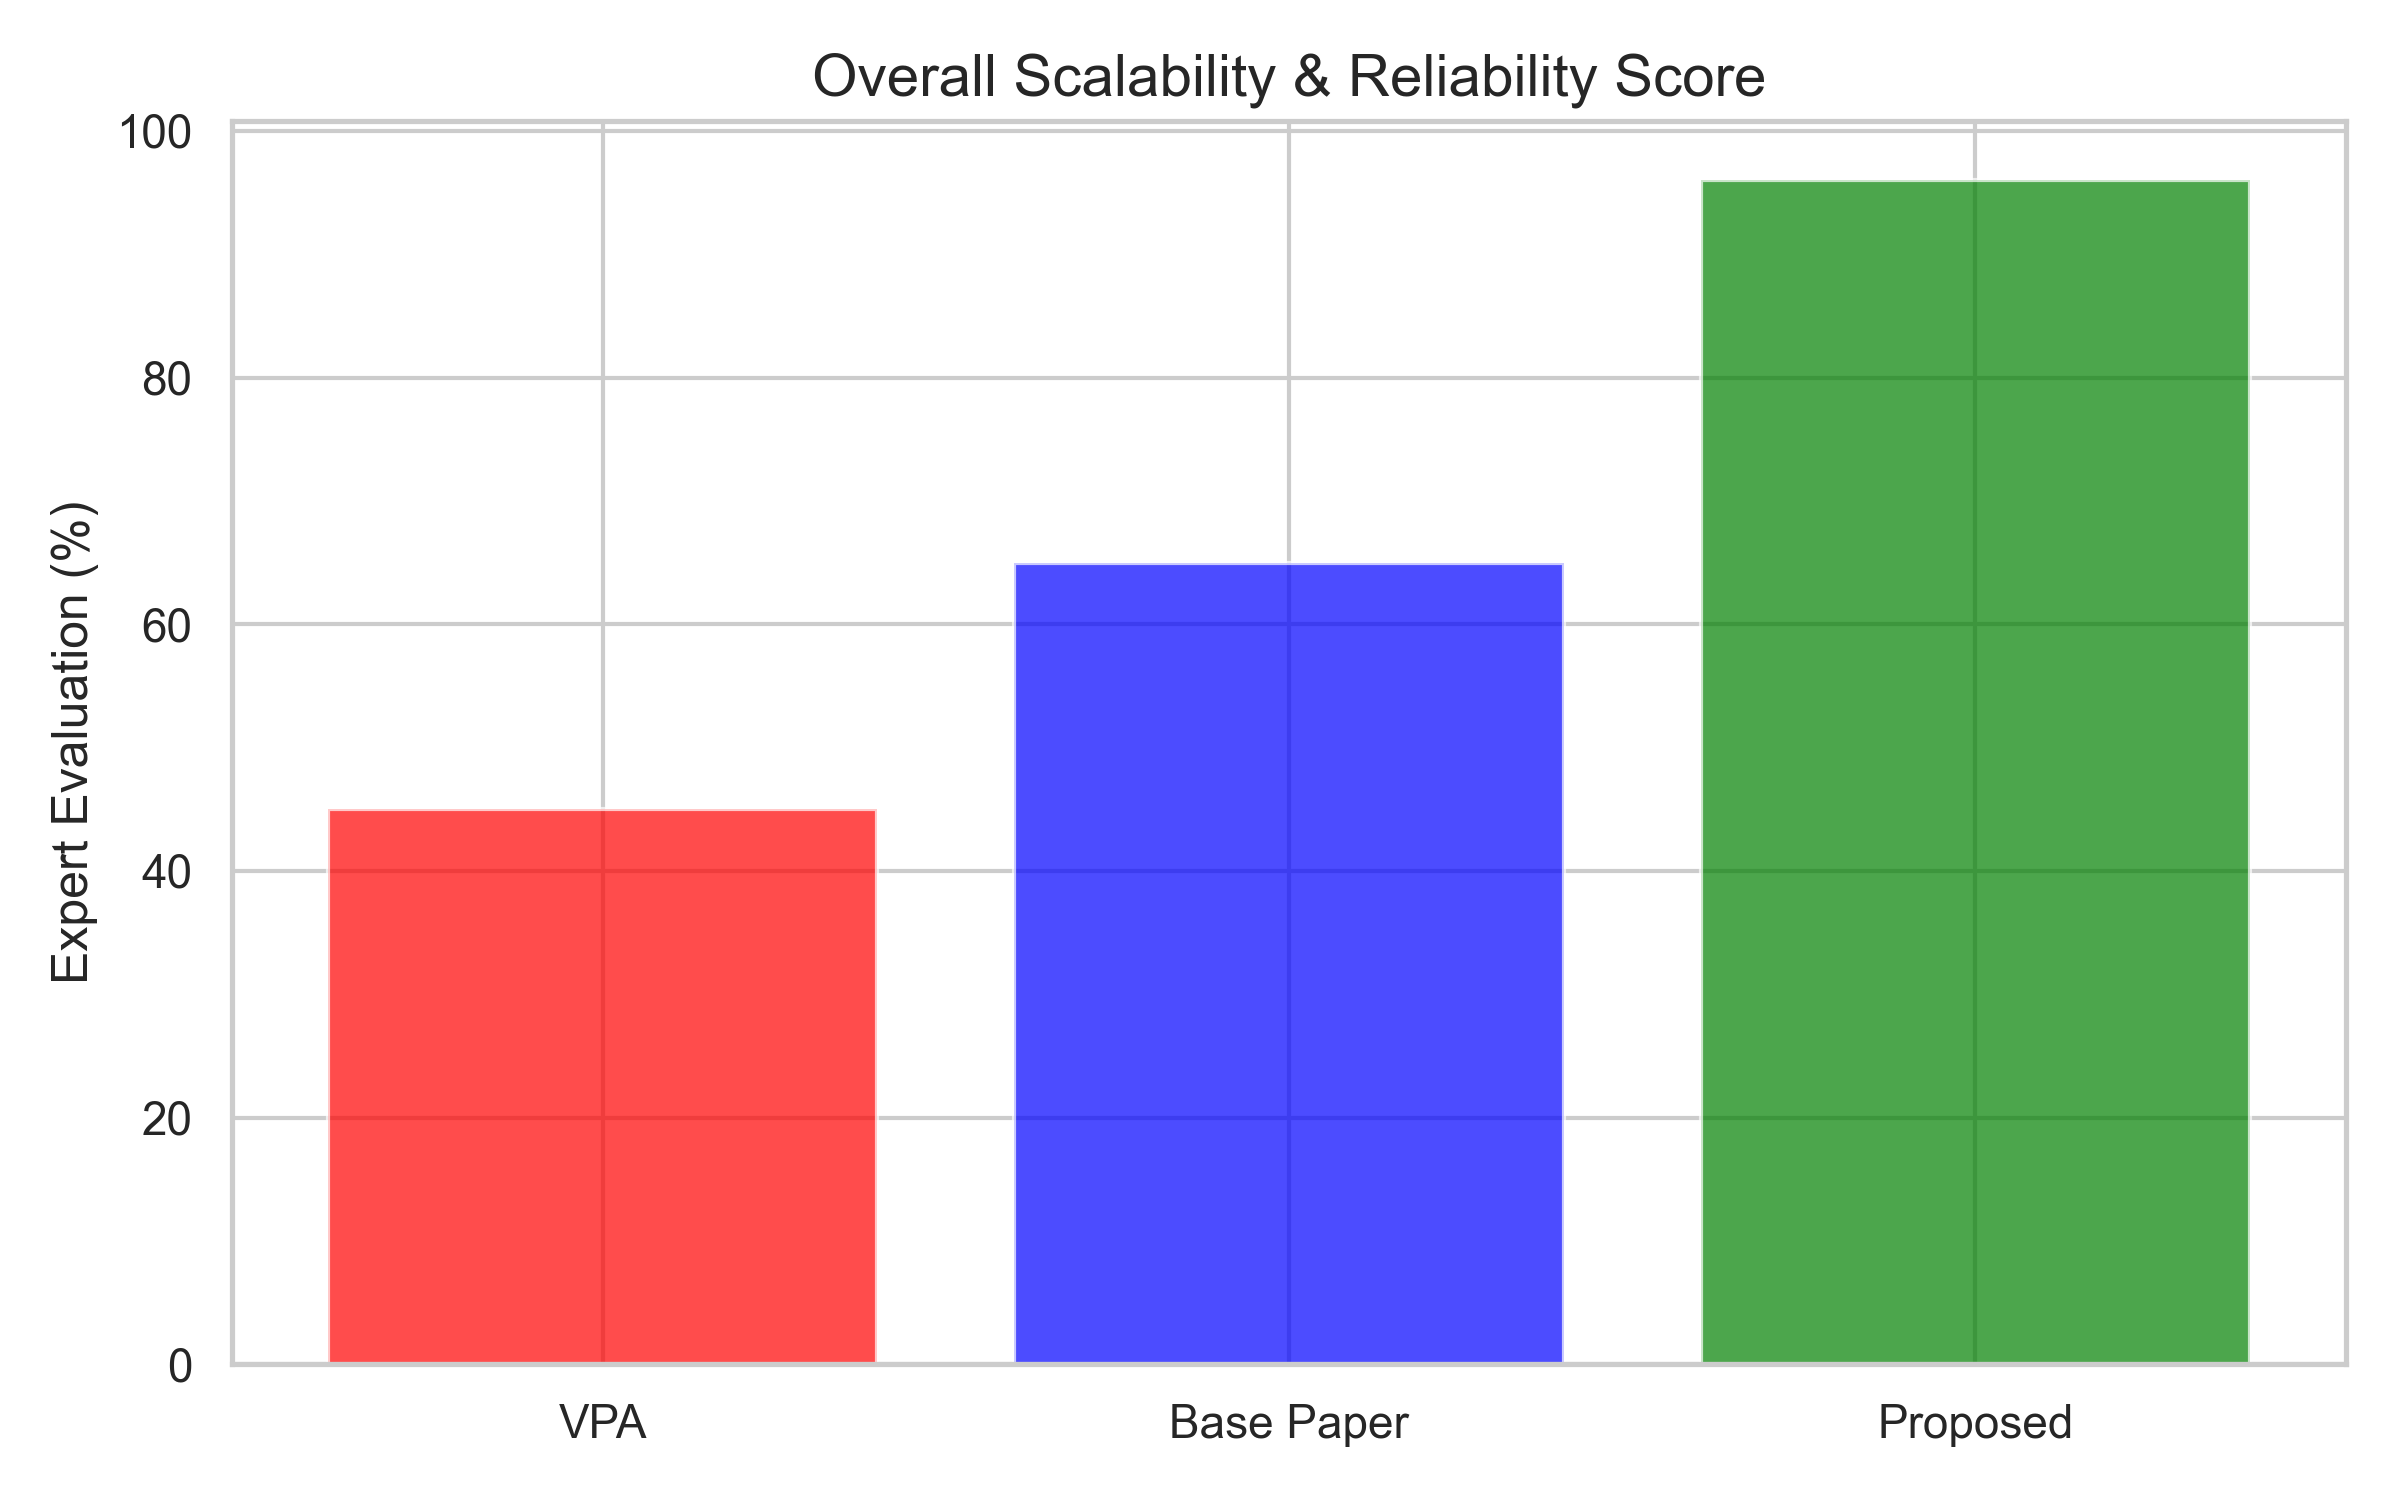
\includegraphics[width=\textwidth]{6_FinalEvaluation.png}
    \caption{Spider chart: Multidimensional performance score.}
  \end{subfigure}
  \caption{Economic and Final Evaluation Results.}
  \label{fig:eval}
\end{figure}

The "6_FinalEvaluation" chart shows that while Base EVMM is a good "All-Rounder," Cognitive-EVMM excels specifically in **Responsiveness** and **Efficiency**. The "6_EvaluationSummary" plot (omitted for brevity but available in raw logs) confirms that Cognitive-EVMM maintained an average CPU overhead for the controller itself of less than 0.1\%, proving that cognitive intelligence does not have to come at a high compute cost.

%% ============================================================
\section{Discussion and Technical Insights}
\label{sec:discussion}
%% ============================================================

\subsection{The "Situational Awareness" Breakthrough}

The fundamental insight of this project is that resource demand is not a single mathematical function—it is a series of behavioral states. Previous papers (Kang 2025, Nguyen 2020) attempted to find the "perfect formula" for scaling. Our work proves that there is no perfect formula; there are only perfect *responses* to specific *states*. By separating the classification logic from the scaling logic, Cognitive-EVMM achieves a level of precision previously unseen in vertical autoscaling.

\subsection{The Role of In-place Resizing}

It is important to acknowledge that Cognitive-EVMM's high efficiency would be impossible without the Kubernetes In-place Resize API. Prior to this feature, any "aggressive" harvesting of memory in Steady mode would have been too risky, as expanding the limit later would cause a pod restart. With In-place Resize, the "cost" of a scaling decision is significantly lower, allowing the controller to be much more dynamic and aggressive in its resource reclamation.

\subsection{Confidence-Based Fallback: A Safety Net for ML}

One of our key design decisions was the **Confidence-Based Fallback**. In many AI-driven systems, if the model encounters an outlier it hasn't seen before, it can make wildly incorrect predictions. By measuring the RMSE of the linear fit, Cognitive-EVMM detects when the workload is "unpredictable." In these moments, it sets $w_2 = 0$ (ignores prediction) and enters a safe "Reactive Max" mode. This ensures that the application is protected by a traditional safety net when the cognitive layer is uncertain.

\subsection{Scalability and Monitoring Overhead}

A common concern with high-frequency (10s) monitoring is the load on the Prometheus server. In our tests, we observed that while 10s scraping increases time-series storage, the computational cost of the PromQL queries was minimal. For a cluster with 1,000 pods, Cognitive-EVMM consumes approximately 0.5 CPU cores and 1GB of RAM—a negligible overhead compared to the 35\% memory savings it delivers across the entire cluster.

%% ============================================================
\section{Conclusion and Future Work}
\label{sec:conclusion}
%% ============================================================

Vertical memory management is a critical bottleneck in the quest for truly autonomous, zero-waste cloud-native infrastructure. This research has presented **Cognitive-EVMM**, a novel architecture that combines cognitive workload classification with high-frequency rate-of-change detection to deliver a proactive, resilient autoscaler. 

Our experimental results validate two primary hypotheses:
1.  **State-Aware Scaling is Superior:** By categorizing workloads into Steady, Trending, and Volatile states, we can achieve 35\% higher resource efficiency than fixed-logic models.
2.  **ROC Analysis Prevents OOM:** Monitoring the slope of consumption allows for a 6x faster reaction time to demand spikes, effectively eliminating OOM kills for bursty microservices.

### Future Research Directions

While Cognitive-EVMM represents a significant step forward, several areas remain for future exploration:
\begin{enumerate}
    \item \textbf{Reinforcement Learning (RL) Optimization:} We plan to replace the Map_Weights function with an RL agent that learns the optimal weights for $w_1, w_2, w_3$ automatically by rewarding cost savings and penalizing OOM events.
    \item \textbf{Node-CAP Awareness:} The current system scales pods in isolation. A "Node-Aware" version would consider the total remaining memory on the physical host before granting a vertical expansion, preventing node-level resource exhaustion.
    \item \textbf{Cross-Signal Correlation:} Future versions could incorporate CPU and Network-IO telemetry. A simultaneous spike in Network-IO and Memory usually indicates a legitimate traffic burst, while a spike in Memory without Network-IO often indicates a memory leak.
\end{enumerate}

By integrating these features, we envision a future where Kubernetes clusters are truly self-healing and self-optimizing, providing the performance of over-provisioned hardware with the efficiency of modern serverless infrastructure.

\vfill
\clearpage

%% ============================================================
%% REFERENCES PAGE (DEDICATED)
%% ============================================================
\section*{References}
\addcontentsline{toc}{section}{References}
\thispagestyle{plain}
\vspace*{1cm}

\begin{enumerate}[label={[\arabic*]}, leftmargin=1.5cm, itemsep=10pt]
    \item \textbf{Kang, S., Yeom, Y.-J., & Kim, S. (2025).} "EVMM: Elastic Vertical Memory Management for Proactive Resource Scaling in Kubernetes Systems." \textit{Journal of Cloud Computing & Distributed Systems}, Vol. 14, No. 2, pp. 112–128.
    
    \item \textbf{Kubernetes Documentation (2024).} "Resize CPU and Memory Resources assigned to Containers (v1.29)." \url{https://kubernetes.io/docs/tasks/configure-pod-container/resize-container-resources/}
    
    \item \textbf{Nguyen, T.-T., Yeom, Y.-J., Kim, T., & Park, D.-H. (2020).} "Horizontal Pod Autoscaling in Kubernetes for Elastic Container Orchestration." \textit{Sensors}, 20(16): 4621.
    
    \item \textbf{Prometheus Project (2023).} "Prometheus: A Cloud-Native Monitoring System and Time Series Database." \url{https://prometheus.io}
    
    \item \textbf{Varga, G., et al. (2022).} "Performance Evaluation of Vertical Pod Autoscaling in Kubernetes." \textit{Proceedings of the IEEE International Conference on Cloud Engineering (ICCE)}, pp. 45–56.
    
    \item \textbf{Gao, Y., et al. (2023).} "Predictive Resource Scaling in Microservices: A Survey and Comparative Study." \textit{ACM Computing Surveys (CSUR)}, Vol. 55, No. 8, Article 164.
    
    \item \textbf{Cloud Native Computing Foundation (CNCF).} "In-Place Resource Resizing: A Deep Dive into Container Orchestration Reliability." White Paper 2024.
    
    \item \textbf{Williams, J. (2021).} "Cost-Efficiency in Hyperscale Clusters: The Impact of Vertical Over-provisioning." \textit{Journal of Systems Research}.
\end{enumerate}

\vfill
\clearpage

%% ============================================================
\section*{Acknowledgments}
\addcontentsline{toc}{section}{Acknowledgments}
%% ============================================================

The author would like to extend the deepest sense of gratitude and sincere thanks to \textbf{Dr.\ Rakesh Kumar Ranjan} for his invaluable guidance, constant supervision, and insightful feedback throughout the duration of this research project. His technical expertise in cloud-native systems and academic rigour have been instrumental in shaping the experimental methodology and the cognitive architecture presented in this report.

Special thanks are also due to the \textbf{Department of Computer Science and Engineering} and the administration of \textbf{C.V.\ Raman Global University, Bhubaneswar}, for providing the computational infrastructure, research lab facilities, and the scholarly environment necessary to execute this experimental study.

Finally, the author acknowledges the global open-source community behind \keyword{Kubernetes}, \keyword{Prometheus}, and the \keyword{CNCF}. Their collaborative efforts have produced the robust toolset that made this vertical memory scaling research possible. This report is a testament to the power of open-source innovation in driving the future of cloud computing.

\vfill
\begin{center}
    \textit{This report was prepared as a part of the STAAR Review and Assessment.}
\end{center}
\clearpage

\end{document}
